\documentclass[pi.tex]{subfile}
\begin{document}
\tikzstyle{menu}=[rectangle, draw=black, rounded corners, fill=blue!40,
        text centered, anchor=north, text=white, text width=4cm]
\tikzstyle{arrow}=[->, >=open triangle 90, thick]
\tikzstyle{line} = [draw, -latex']

\chapter{PERANCANGAN DAN IMPLEMENTASI}
Dalam bab ini akan dijelaskan lebih lanjut mengenai bagaimana perancangan dan implementasi bahasa pemrograman Haskell dalam pembuatan aplikasi desktop GUI menggunakan metode pemrograman FRP dan teknologi website.

\section{Gambaran Umum Aplikasi}
Seperti yang telah dijelaskan pada bab terdahulu, komputasi awan (\emph{cloud computing} atau biasa kita sebut \emph{cloud}  merupakan sebuah teknologi baru dalam dunia komputer khususnya dalam bidang sumber daya IT yaitu server. Hampir seluruh server yang digunakan oleh penyedia layanan teknologi informasi mulai memanfaatkan teknologi awan ini untuk mereduksi besaran biaya yang umumnya dikeluarkan apabila menggunakan arsitektur komputer tanpa awan. Di Indonesia, beberapa penyedia layanan IT baik berupa layanan ke konsumen maupun sesama penyedia jasa IT juga mulai melirik menggunakan teknologi awan ini. Sebagai contoh antara lain tokopedia.com, Go-Jek, bukalapak.com dan penyedia jasa IT lainnya berlomba-lomba untuk melakukan reduksi biaya yang timbul agar mendapat keuntungan maksimal dengan memindahkan sebagian infrastruktur IT nya ke layanan awan.

Selain dari sisi pengguna layanan komputasi awan, penyedia jasa komputasi awan publik sampai saat ini mulai tumbuh dan bersaing satu dengan lainnya untuk menarik perhatian konsumennya. Penyedia jasa komputasi awan publik antara lain, Amazon AWS, Google Cloud, Alibaba Cloud, yang berbasis penggunaan perjam, maupun DigitalOcean, Vultr, CloudKilat, yang berbasis penggunaan perbulan. Dalam penulisan kali ini yang jadi pembahasan adalah mengenai Amazon AWS atau dapat dikenal juga dengan nama \emph{Amazon Web Service}.

Jasa yang dihitung pada Aplikasi adalah jasa yang masuk ke dalam jenis \emph{On-Demand} yaitu jasa yang pembayarannya dibebankan kepada pengguna sesuai dengan jumlah lama penggunaan atas jasa tersebut. Dengan Aplikasi ini, pengguna pemula diharapkan tidak memerlukan koneksi internet maupun mendaftar sebagai member AWS untuk mengetahui estimasi biaya jasa AWS yang ingin digunakan.

Aplikasi bersifat dinamis, yaitu kalkulasi dilakukan secara \emph{real-time} pada saat pengguna menginput parameter-parameter terhadap atribut jasa AWS yang digunakan. Perhitungan secara \emph{real-time} ini menggunakan konsep FRP yang ada pada pustaka Reflex dan Reflex-Dom, sehingga pembaharuan terhadap DOM berupa hasil kalkulasi terlihat terjadi seketika.

\section{Kebutuhan Perangkat dan Instalasi Aplikasi}
Dalam Penulisan Ilmiah ini, tidak semua perangkat komputer dapat menjalankannya. Hal ini dipengaruhi oleh spesifikasi perangkat keras \emph{hardware} dan spesifikasi perangkat lunak \emph{software} mesin tempat dimana Aplikasi akan dijalankan.

Selain dar kebutuhan perangkat, Aplikasi tidak dapat langsung digunakan, melainkan harus melalui tahapan instalasi terlebih dahulu. Kebutuhan akan penjelasan bagaimana cara melakukan instalasi Aplikasi di sebuah mesin yang sudah dianggap sesuai dengan spesifikasi minimal sangat diperlukan untuk meminimalisir kesalahan pada saat aplikasi dijalankan.

Oleh karena itu, berikut ini akan dijelaskan apa saja kebutuhan perangkat dan bagaimana cara melakukan instalasi Aplikasi di sebuah sistem operasi OS X.
\subsection{Kebutuhan Minimal dan Maksimal Perangkat}\hspace{5pt}
Kebutuhan minamal perangkat keras dan lunak untuk menjalankan Aplikasi adalah pada Tabel 3.1.

\begin{table}[h]
  \centering
\begin{tabular}{ |p{3cm}||p{6cm}|}
  
  \hline
  \multicolumn{2}{|c|}{Minimum Requirement} 
  \\ \hline
  Name & Specification \\
  \hline
  Sistem Operasi : & macOS Sierra \\
  Processor : & 2.4 GHz Intel Core 2 Duo \\
  Memory : & 4GB \\
  Graphics : & NVIDIA GeForce 320M 256MB \\
  \hline
  
\end{tabular}
\caption{Kebutuhan Minimal}
\end{table}

\hspace{5pt}Kebutuhan minimal diperlukan agar pengguna mengetahui apakah perangkat yang dimilikinya mampu untuk menjalankan Aplikasi. Kemampuan Aplikasi berjalan pada spesifikasi perangkat pada tingkat minimal menunjukkan bahwa jalannya Aplikasi tidak akan mengganggu atau membuat aktivitas perangkat menjadi terganggu.

\begin{table}[h]
  \centering
\begin{tabular}{ |p{3cm}||p{6cm}|}
  \hline
  \multicolumn{2}{|c|}{Recommended Requirement} 
  \\ \hline
  Name & Specification \\
  \hline
  Sistem Operasi : & macOS Sierra \\
  Processor : & 2.8 GHz Intel Core i7 \\
  Memory : & 16GB \\
  Graphics : & NVIDIA GeForce GT 750M 2048MB \\
  \hline
  
\end{tabular}

\caption{Kebutuhan Yang Direkomendasikan}
\end{table}

\hspace{5pt}Kebutuhan yang direkomendasikan seperti pada Tabel 3.2, diperlukan agar baik pengguna maupun pengembang mengetahui perangkat mana yang dapat menghasilkan performa yang optimal ketika Aplikasi sedang dijalankan.

\hspace{5pt}Dari Tabel 3.1 dan Tabel 3.2, sistem operasi berperan penting dalam penentuan spesifikasi sebuah Aplikasi. Hal ini dikarenakan apabila jenis perangkat keras telah terpenuhi namun sistem operasi tidak terpenuhi, Aplikasi tidak dapat dijalankan.

\subsection{Instalasi Aplikasi}
\hspace{5pt}Instalasi Aplikasi dilakukan melalui beberapa tahapan, yaitu:
\subsubsection{Instalasi XCode dan XCode Command Line Tools}\hspace{10pt}
\hspace{10pt}Instalasi XCode dapat dilakukan dengan membuka App Store pada menu \emph{dock} MacOS (Letak \emph{dock} ada dibagian bawah Desktop) seperti pada Gambar 3.1.

  \begin{figure}[H]
      \centering
  
\includegraphics{appStore}
  \caption[Ikon AppStore]{Ikon AppStore}

  \end{figure}

  \hspace{10pt}Tekan ikon App Store dua kali sehingga akan muncul jendela App Store, kemudian cari aplikasi XCode pada menu pencarian seperti pada Gambar 3.2.

  \begin{figure}[H]
      \centering
  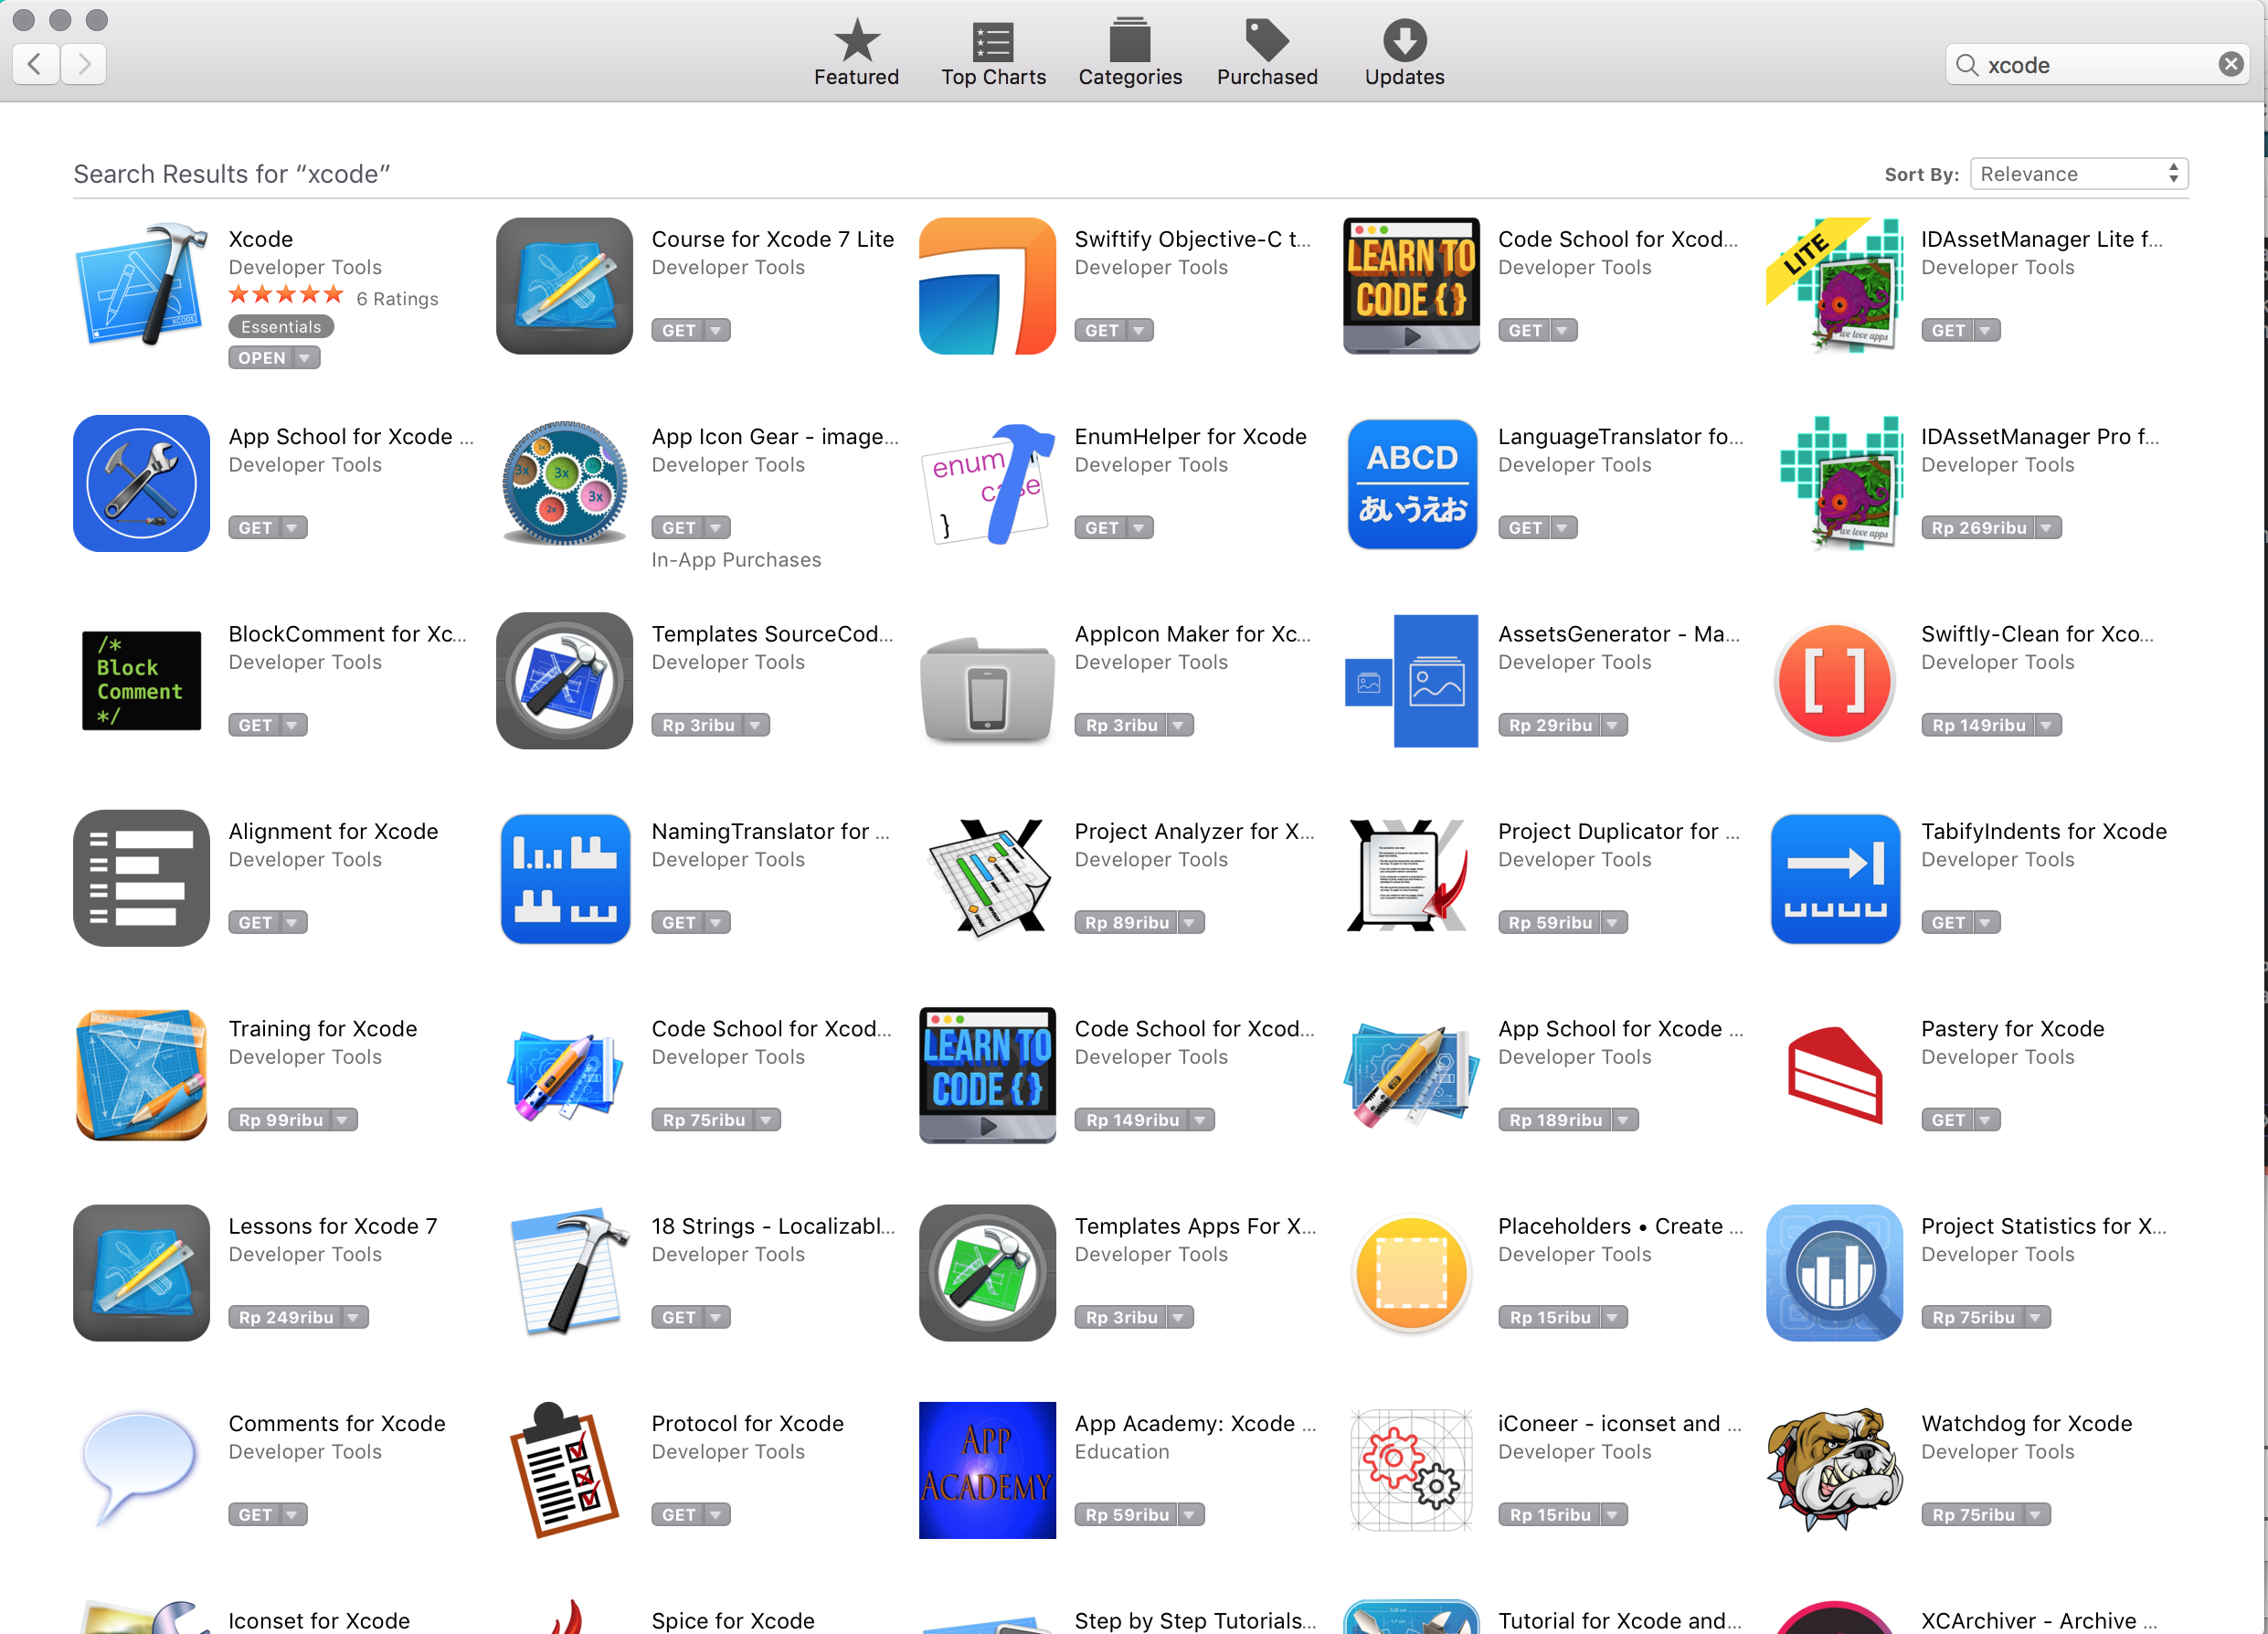
\includegraphics[width=\textwidth]{appStore1}
  \caption[Jendela AppStore]{Jendela AppStore}

  \end{figure}

  \hspace{10pt}Pasang XCode pada MacOS dengan menekan tombol GET. Gambar 3.3 adalah contoh tampilan ikon XCode yang dibutuhkan:
  

  \begin{figure}[H]
      \centering
  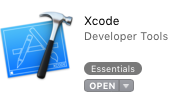
\includegraphics[width=\textwidth]{xcode.png}
  \caption[Ikon XCode]{Ikon XCode}
  \end{figure}

  \hspace{10pt}Setelah selesai melakukan instalasi, buka terminal MacOS dan ketikkan perintah \fhaskell{xcode-select --install} pada terminal untuk memasang program tambahan yaitu \emph{XCode Command Line} yang berfungsi untuk melakukan kompilasi program di terminal. Hal ini dibutuhkan karena Aplikasi berbasis Haskell akan dikompilasi di terminal.

  \begin{figure}[H]
      \centering
  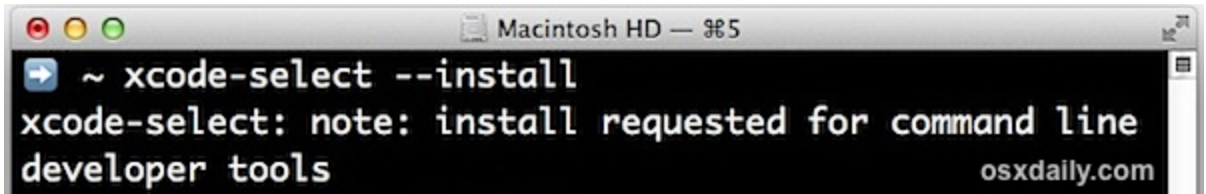
\includegraphics[width=\textwidth]{xcodeCmd}
  \caption[Tampilan Instalasi Command Line]{Tampilan Instalasi Command Line}
  \end{figure}

  \hspace{10pt}Kemudian apabila \emph{XCode Command Line} belum terinstall, maka akan muncul jendela konfirmasi terkait instalasi \emph{XCode Command Line} seperti pada Gambar 3.5. Klik pada tombol install untuk melakukan instalasi xcode command line tools dan kemudian tunggu proses instalasi tersebut hingga selesai seperti pada Gambar 3.6.

 \begin{figure}[H]
      \centering
  
\includegraphics[width=\textwidth]{xcodeCmd1}
  \caption[Tampilan Jendela Konfirmasi]{Tampilan Jendela Konfirmasi}
 \end{figure}

  \begin{figure}[H]
      \centering
  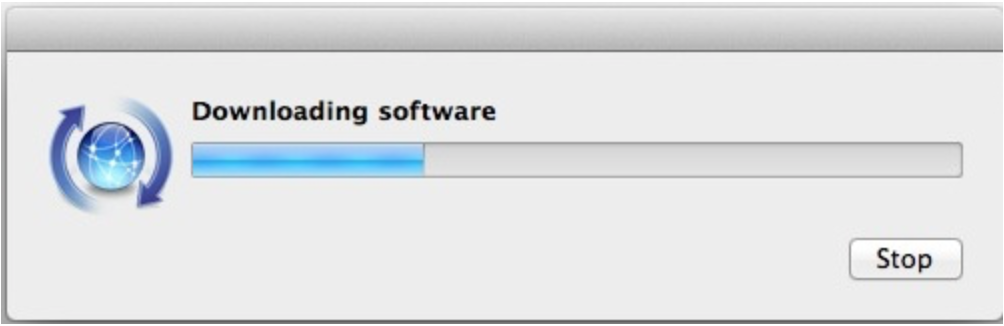
\includegraphics[width=\textwidth]{xcodeCmd2}
  \caption[Tampilan Proses Instalasi Command Line]{Tampilan Proses Instalasi Command Line}
  \end{figure}

  \hspace{10pt}Apabila telah berhasil terpasang, ketik perintah \fhaskell{xcode-select -p} untuk memastikan instalasi telah berhasil. Dengan terpasangnya XCode dan XCode Command Line, maka GHC dapat mengambil beberapa pustaka bawaan yang terpasang pada sistem operasi OS X dan menggunakannya untuk membuat aplikasi yang dapat berjalan di atas sistem operasi tersebut.
  
\subsubsection{Instalasi GHC sebagai alat kompilasi dan Cabal sebagai manajemen paket}\hspace{10pt}
Untuk mamasang GHC pada MacOS, dapat dilakukan dengan cara mengunduh GHC melalui situs resminya[8] pada bagian \emph{Binary Package} seperti pada Gambar 3.7.

  \begin{figure}[H]
      \centering
  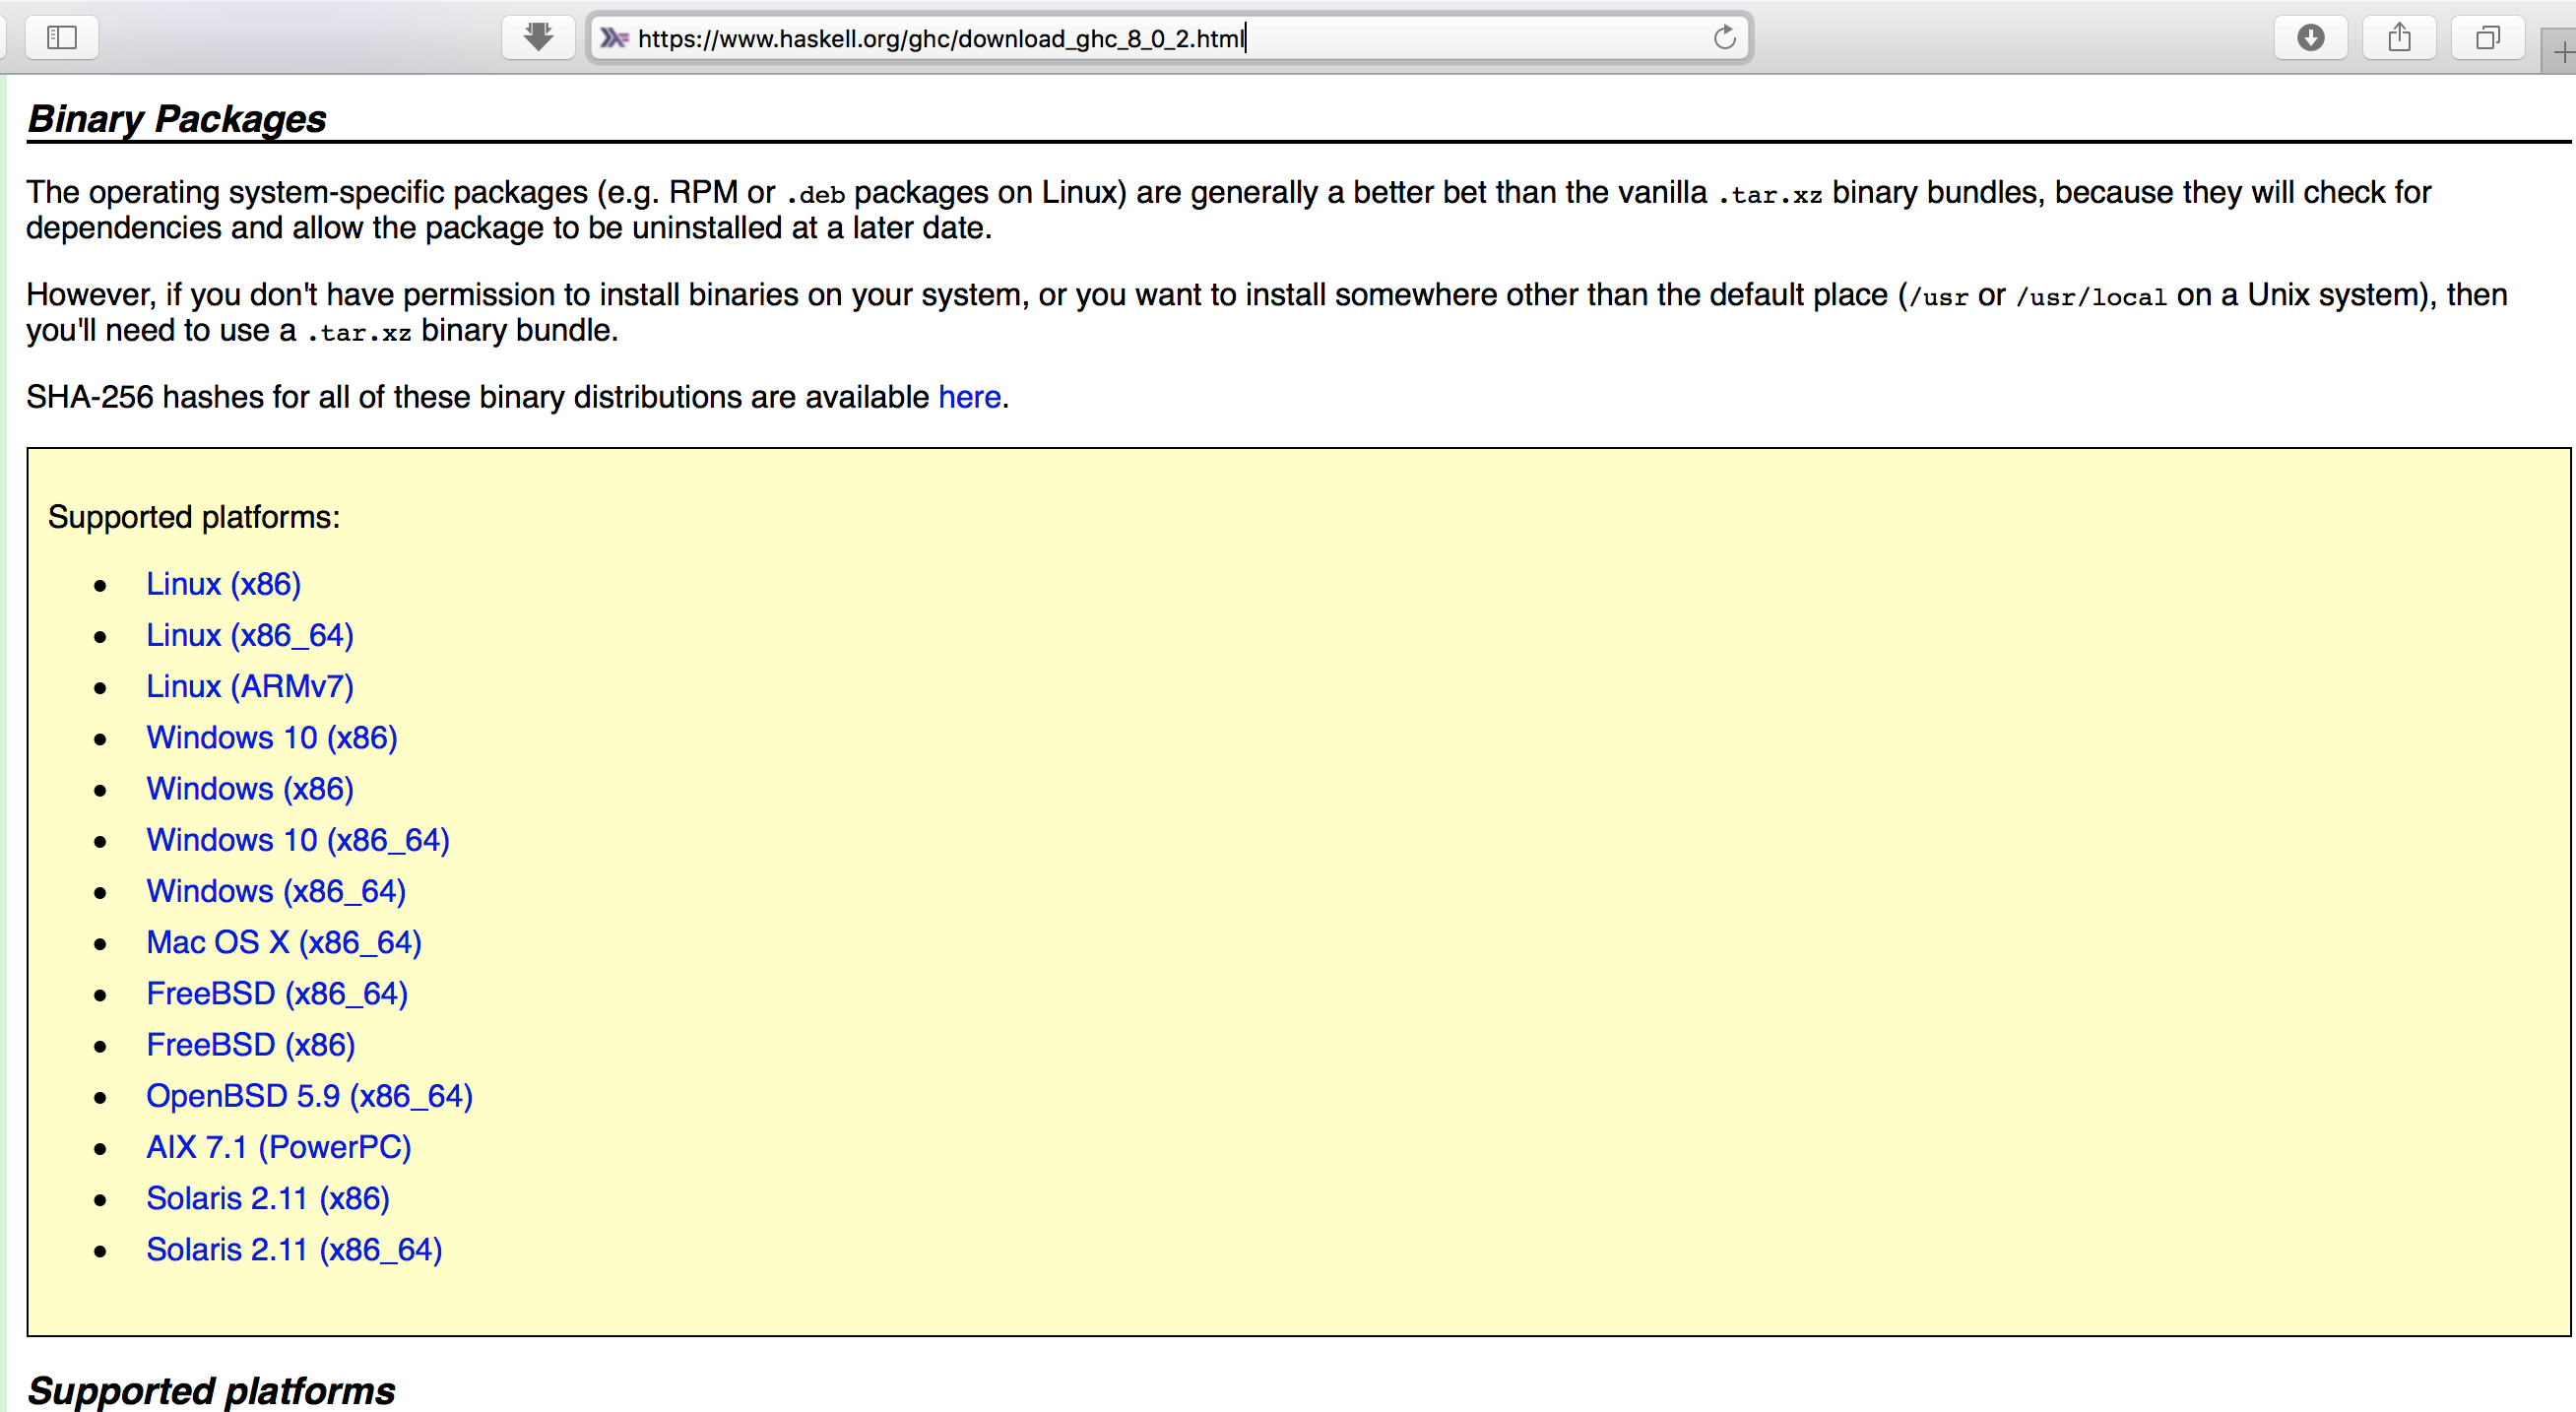
\includegraphics[width=\textwidth]{ghc}
  \caption[Tautan Lokasi Binary GHC]{Tautan Lokasi Binary GHC}
  \end{figure}

    \begin{figure}[H]
      \centering
  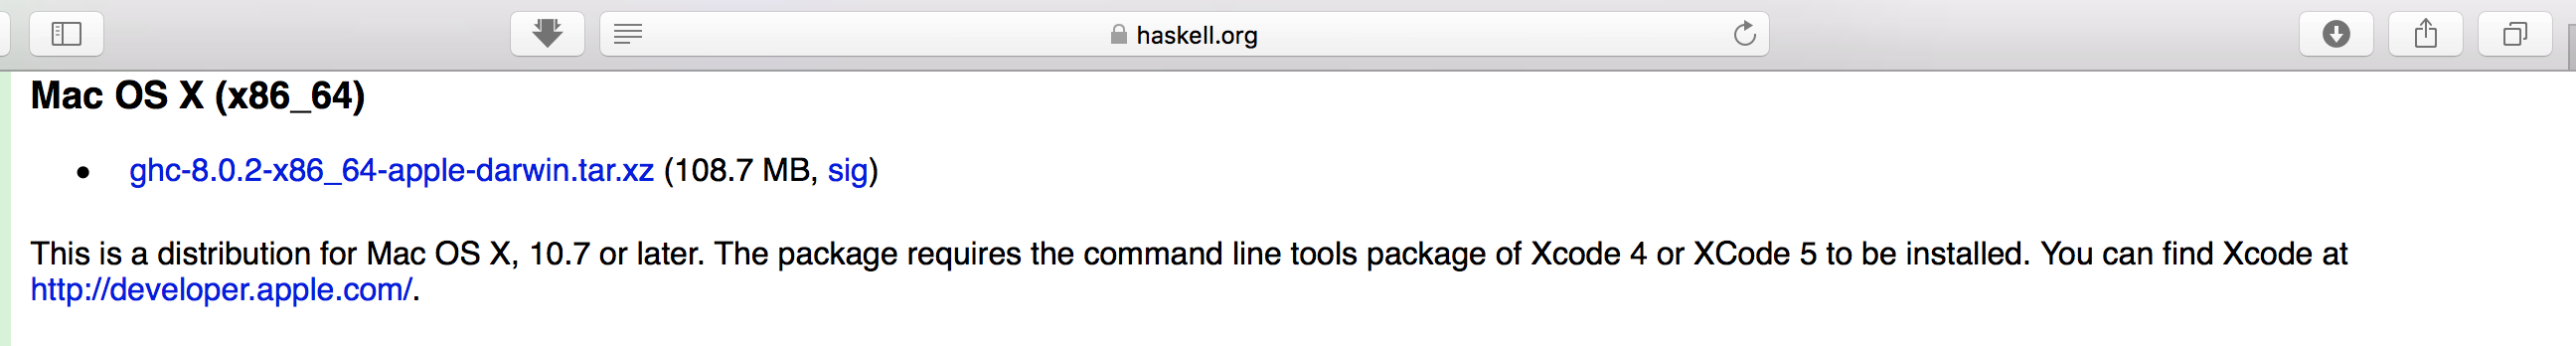
\includegraphics[width=\textwidth]{ghc1}
  \caption[Tautan Lokasi Binary GHC Untuk OS X]{Tautan Lokasi Binary GHC Untuk OS X}
  \end{figure}


    \hspace{10pt}Download file \emph{binary} untuk Mac OS X (lihat Gambar 3.8) kemudian \emph{extract} isi dari file tersebut dengan menjalankan perintah \fhaskell{tar zxfv ghc-8.0.2-x86\_64-apple-darwin.tar.xz}. Pindah kedalam direktori dengan perintah \fhaskell{cd ghc-8.0.2} dan jalankan \emph{script installer} dengan mengetikan perintah \fhaskell{./configure}. Proses konfigurasi akan dilakukan seperti pada Gambar 3.9.

    \hspace{10pt}Apabila konfigurasi telah selesai, jalankan perintah \fhaskell{make install} pada terminal seperti pada Gambar 3.10. Apabila telah selesai, maka program GHC akan dipasang dilokasi folder \fhaskell{/usr/local}.
  \begin{figure}[H]
      \centering
  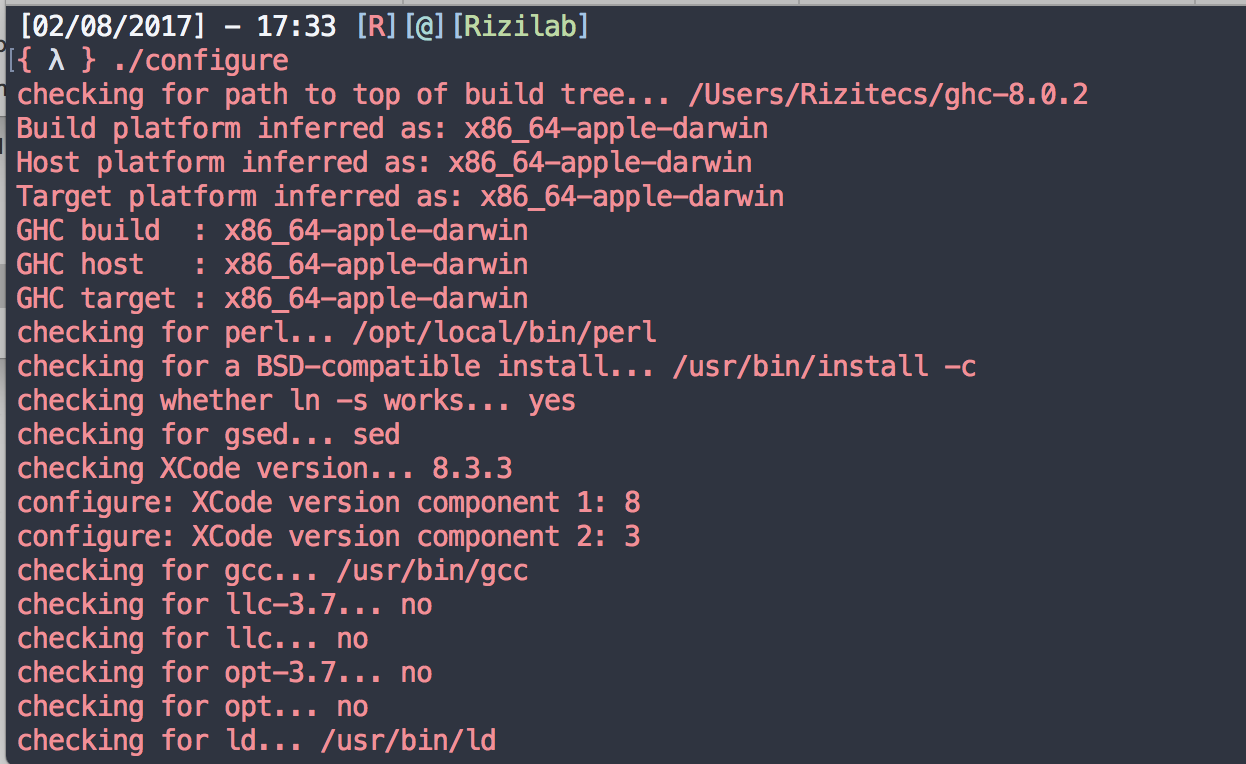
\includegraphics[width=\textwidth]{ghc2}
  \caption[Tampilan Konfigurasi \emph{Script}]{Tampilan Konfigurasi \emph{Script}}
  \end{figure}


  \begin{figure}[H]
      \centering
  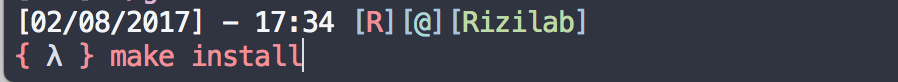
\includegraphics[width=\textwidth]{ghc3}
  \caption[Tampilan Perintah Install GHC]{Tampilan Perintah Install GHC}
  \end{figure}

  \hspace{10pt}Selanjutnya untuk manajemen paket pada pengembangan Aplikasi, dibutuhkan program bernama Cabal. Pemasangan Cabal dapat dilakukan dengan mengunduh dari situs Cabal[9] dan pilih Cabal library serta cabal-install tools. Extract cabal-install dan jalankan shell script bernama \emph{bootstrap.sh} dimana skrip ini mengunduh dan memasang semua kebutuhan paket yang akan digunakan oleh program cabal-install.
  
\subsubsection{Instalasi Aplikasi dari kode sumber}\hspace{10pt}
Unduh kode sumber dari Aplikasi di \url{https://github.com/Rizary/awspi} dengan cara menekan tombol \fhaskell{Clone or download} dan pilih opsi \fhaskell{Download ZIP} seperti pada Gambar 3.11.

\begin{figure}[H]
    \centering
  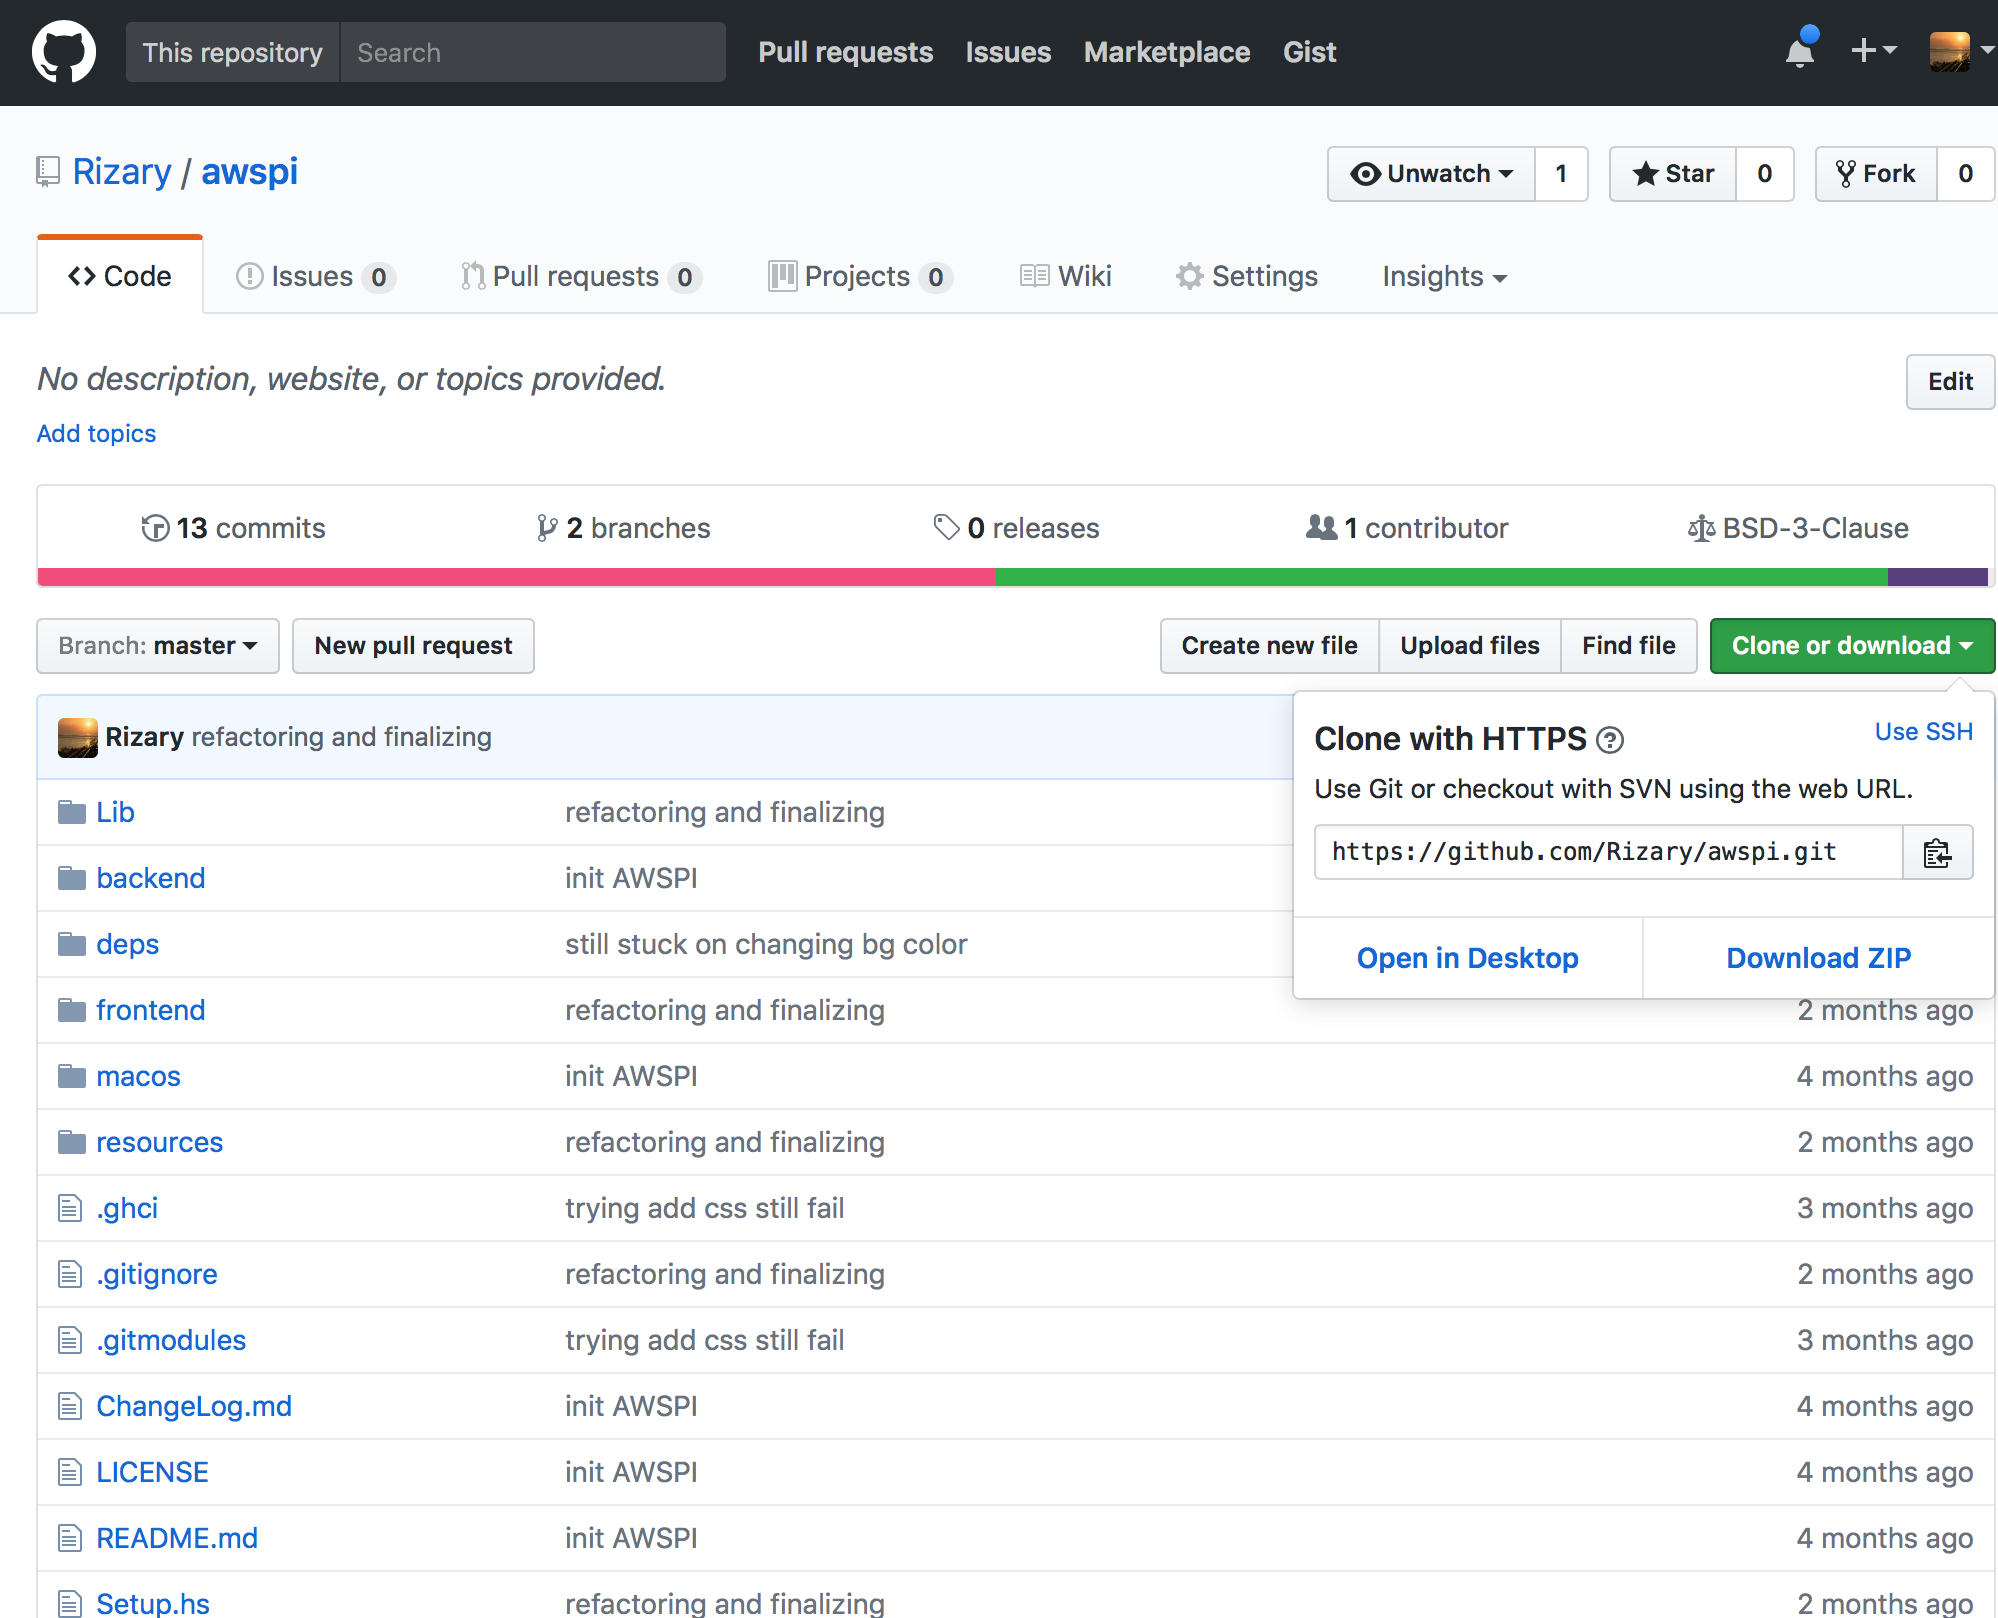
\includegraphics[width=15cm, height=10cm]{source}
  \caption[Tampilan Halaman \emph{Download} Kode Sumber]{Tampilan Halaman \emph{Download} Kode Sumber}
  \end{figure}


\hspace{10pt}Buka file dengan ekstensi \fhaskell{.zip} tersebut dan \emph{extract} file kemudian pindah kedalam direktori kode dengan mengetik perintah \fhaskell{cd awspi} pada terminal. Setelah berhasil masuk kedalam folder kode sumber, jalankan perintah \fhaskell{cabal new-build} pada terminal untuk melakukan kompilasi terhadap kode sumber Aplikasi tersebut.

  \hspace{10pt}Setelah proses kompilasi berhasil, file \emph{binary} dari aplikasi akan terletak pada folder \url{./dist-newstyle/build/x86_64-osx/ghc-8.0.2/awspi-0.0.0.1/build/} dalam bentuk ekstensi \fhaskell{.app}. Klik 2 kali pada file tersebut untuk menjalankan Aplikasi. Aplikasi yang berhasil dijalankan akan tampak seperti Gambar 3.12.
  
  \begin{figure}[H]
    \centering
  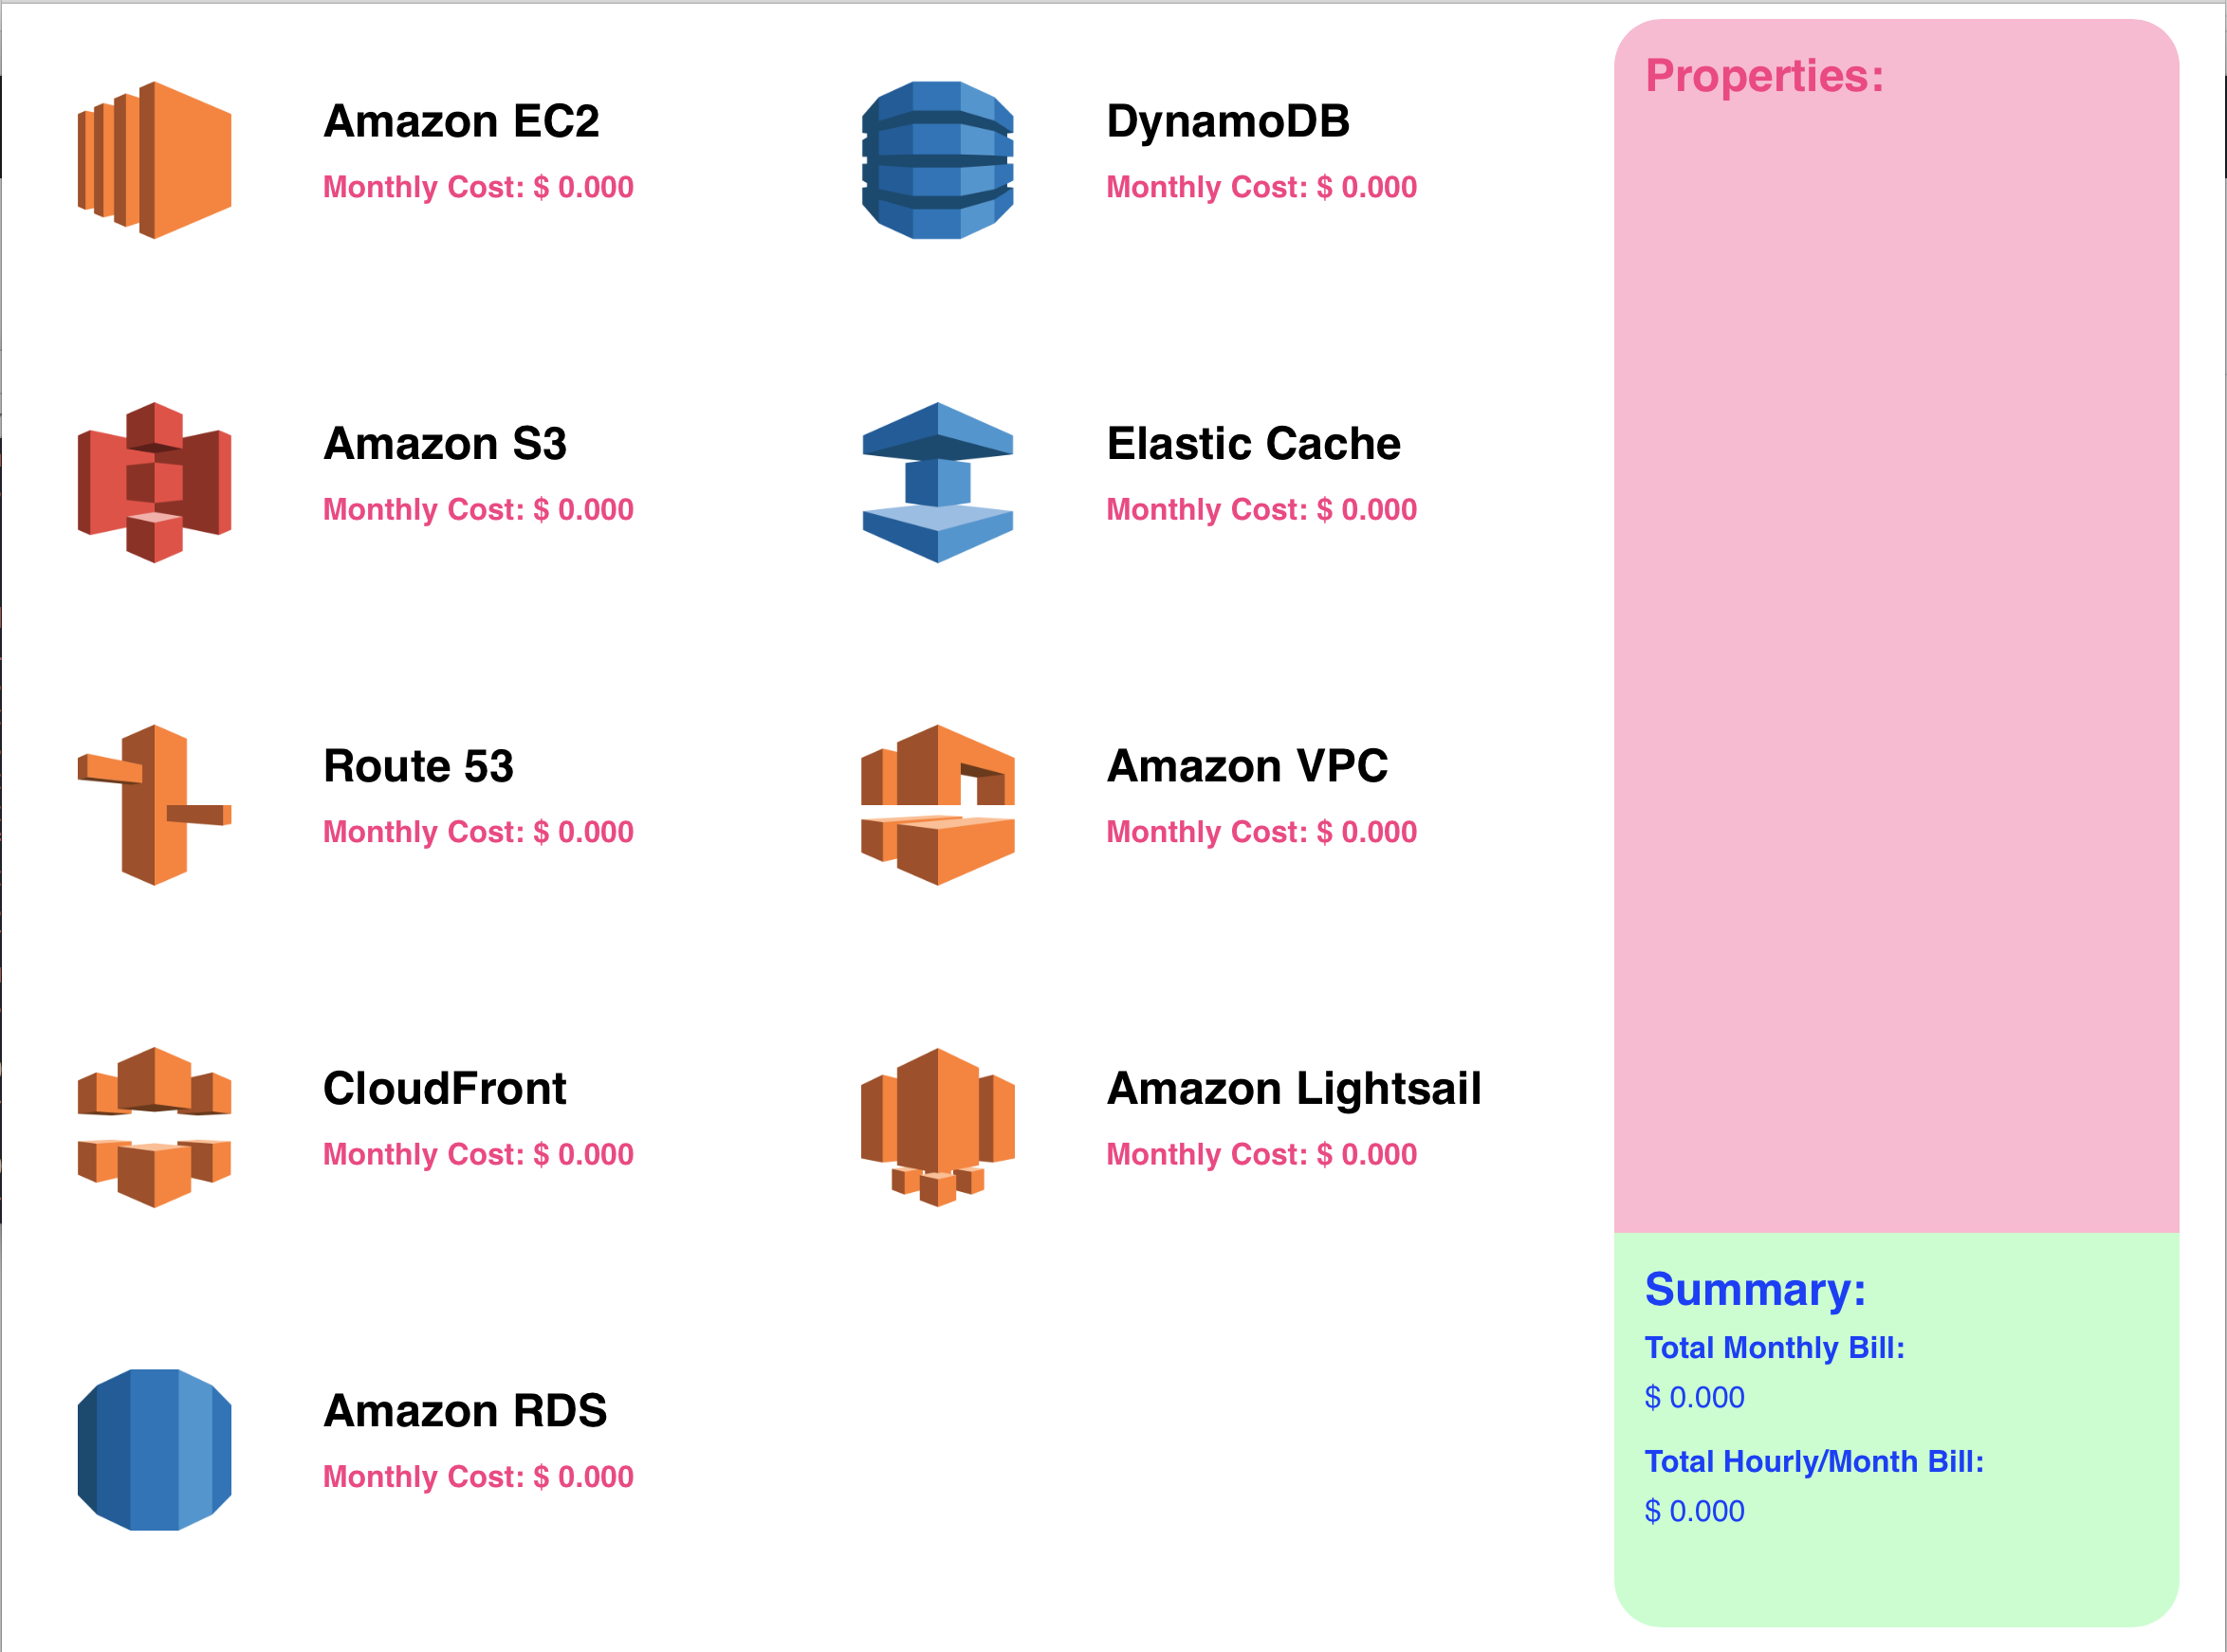
\includegraphics[width=7cm, height=3.5cm]{awspi.png}
  \caption[Tampilan Awal Aplikasi]{Tampilan Awal Aplikasi}
  \end{figure}

  \hspace{10pt}Apabila sudah sesuai dengan gambar diatas, maka Aplikasi sudah dapat digunakan.

\section{Tahapan Pembuatan Dan Algoritma Aplikasi}
\subsection{Tahapan Pembuatan Aplikasi}\hspace{5pt}
Dalam membuat Aplikasi, tahapan yang dilakukan adalah merancang dan membuat desain. Perancangan Aplikasi pada penulisan ilmiah ini, salah satu metode yang digunakan adalah merancang struktur navigasi. Struktur navigasi merupakan sebuah alur dari suatu aplikasi yang berisi rancangan rantai kerja dari beberapa area yang berbeda dan dapat membantu mengorganisasikan seluruh elemen pembuatan aplikasi dengan memberikan perintah atau pesan antar elemen tersebut.

\hspace{10pt}Pada pembuatan Aplikasi, struktur navigasi digambarkan seperti pada Gambar 3.13.

\begin{figure}[H]
  \centering
  \begin{tikzpicture}[node distance=2cm]
    \node (main)[menu]
          {
            \textbf{Menu Utama}
          };
    \node (prop)[menu,below of=main]
          {
            \textbf{Menu Properti}
          };
    \node (RDS)[menu,left of=prop, xshift=-4cm]
          {
            \textbf{Properti \\ Amazon RDS}
          };
    \node (CF)[menu,below of=RDS]
          {
            \textbf{Properti CloudFront}
          };
    \node (R53)[menu,below of=CF]
          {
            \textbf{Properti Route53}
          };
    \node (S3)[menu,below of=R53]
          {
            \textbf{Properti Amazon S3}
          };
    \node (EC2)[menu,below of=S3]
          {
            \textbf{Properti \\ Amazon EC2}
          };          
    \node (DDB)[menu,right of=prop, xshift=4cm]
          {
            \textbf{Properti \\ DynamoDB}
          };
    \node (EC)[menu,below of=DDB]
          {
            \textbf{Properti \\ ElasticCache}
          };
    \node (VPC)[menu,below of=EC]
          {
            \textbf{Properti \\ Amazon VPC}
          };
    \node (LS)[menu,below of=VPC]
          {
            \textbf{Properti \\ Amazon LightSail}
          };
    \node (Summ)[menu,below of=prop]
          {
            \textbf{Menu Summary}
          };

          \path[line] (main.south) -- (prop.north);
          \path[line] (prop.west) -- (CF.east);
          \path[line] (prop.west) -- (R53.east);
          \path[line] (prop.west) -- (S3.east);
          \path[line] (prop.west) -- (EC2.east);
          \path[line] (prop.west) -- (RDS.east);
          \path[line] (prop.east) -- (DDB.west);
          \path[line] (prop.east) -- (EC.west);
          \path[line] (prop.east) -- (VPC.west);
          \path[line] (prop.east) -- (LS.west);
          \path[line] (prop.south) -- (Summ.north);
          
  \end{tikzpicture}
  \caption[Struktur Navigasi Aplikasi]{Struktur Navigasi Aplikasi AWS}
\end{figure}

\hspace{10pt}Dari struktur navigasi diatas, dapat diketahui bahwa pembuatan Aplikasi menggunakan struktur navigasi Hirarki karena jendela utama dari Aplikasi terletak pada Menu Utama berfungsi sebagai \emph{Master Page}. Menu Utama tersebut terhubung kepada masing-masing properti yaitu kedalam Menu Properti sebagai \emph{Slave Page} dan berisi properti Amazon RDS, CloudFront, Route53, Amazon S3, Amazon EC2, DynamoDB, ElasticCache, Amazon VPC, dan Amazon LightSail. Menu properti tersebut terhubung dan bergantung pada Menu Utama dan akan berubah seiring dengan ikon yang dipilih oleh pengguna nantinya.

\hspace{10pt}Menu Utama yang dimaksud dalam struktur navigasi diatas berisikan ikon-ikon jasa AWS yang dapat dipilih sehingga akan menampilkan isi dari Menu Properti terkait. Contoh menu utama dalam desain adalah seperti pada Gambar 3.14.

  \begin{figure}[H]
      \centering
  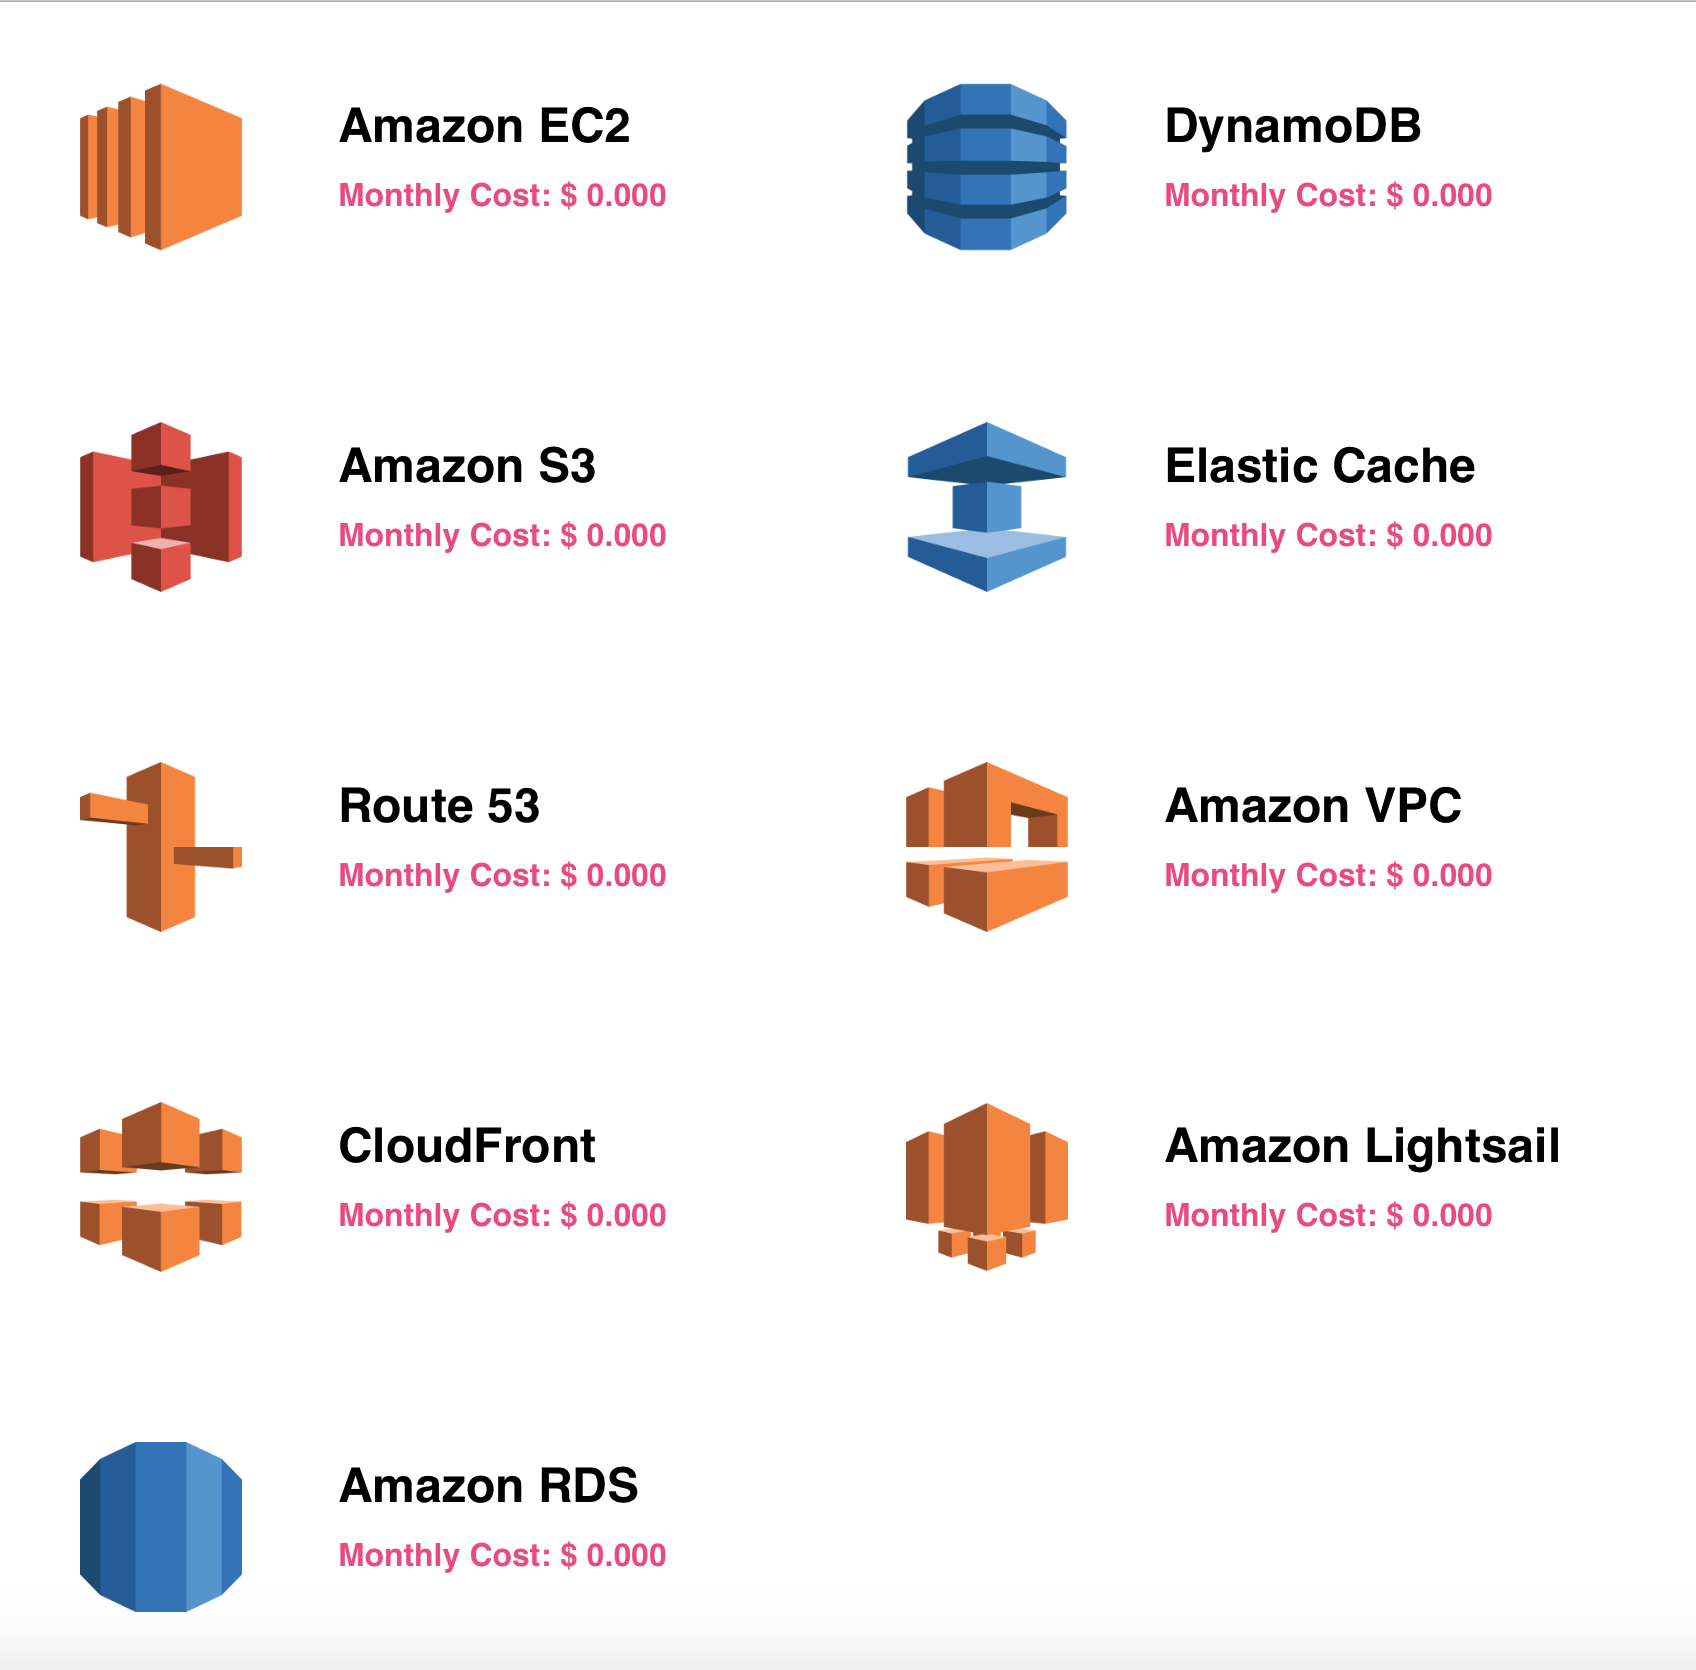
\includegraphics[width=10cm, height=10cm]{aws3.png}\\
  \caption[Menu Utama Aplikasi]{Menu Utama Aplikasi AWS}
  \end{figure}

  \hspace{10pt}Menu utama merupakan acuan untuk menampilkan menu properti yang terletak di sebelah kanan Aplikasi. Ikon-ikon jasa AWS pada Menu Utama merupakan jasa AWS yang paling banyak digunakan oleh pengembang dalam memanfaatkan teknologi \emph{cloud} guna mendukung aplikasi yang dibuat.

  \hspace{10pt}Tampilan menu properti dapat dilihat seperti pada Gambar 3.15. Menu summary tidak dapat berubah, sehingga bersifat statis mengikuti menu utama. Dengan demikian, struktur navigasi yang sesuai untuk pembuatan aplikasi ini adalah non-linier karena dalam struktur ini terdapat percabangan, namun tidak adanya master maupun slave pada halaman tersebut.

    \begin{figure}[H]
      \centering
  
\includegraphics[width=8cm, height=10cm]{aws4.png}\\
  \caption[Menu Properties Aplikasi]{Menu Properties Aplikasi AWS}
  \end{figure}

    \hspace{10pt}Untuk membuat desain Aplikasi, penelitian ilmiah ini menggunakan aplikasi pendukung prototipe bernama Sketch pada MacOS dengan menggunakan metode desain 8pt (\emph{8pt Design}), yaitu jarak spasi antara satu ikon / gambar dengan yang lainnya berjarak 8 point atau kelipatan 8 (termasuk didalamnya kelipatan 2 dan 4). Hal ini akan memudahkan dalam penggunaan di dalam beberapa resolusi layar. Hasil final terhadap desain adalah seperti pada Gambar 3.16 dan 3.17.
    \begin{figure}[H]
      \centering
  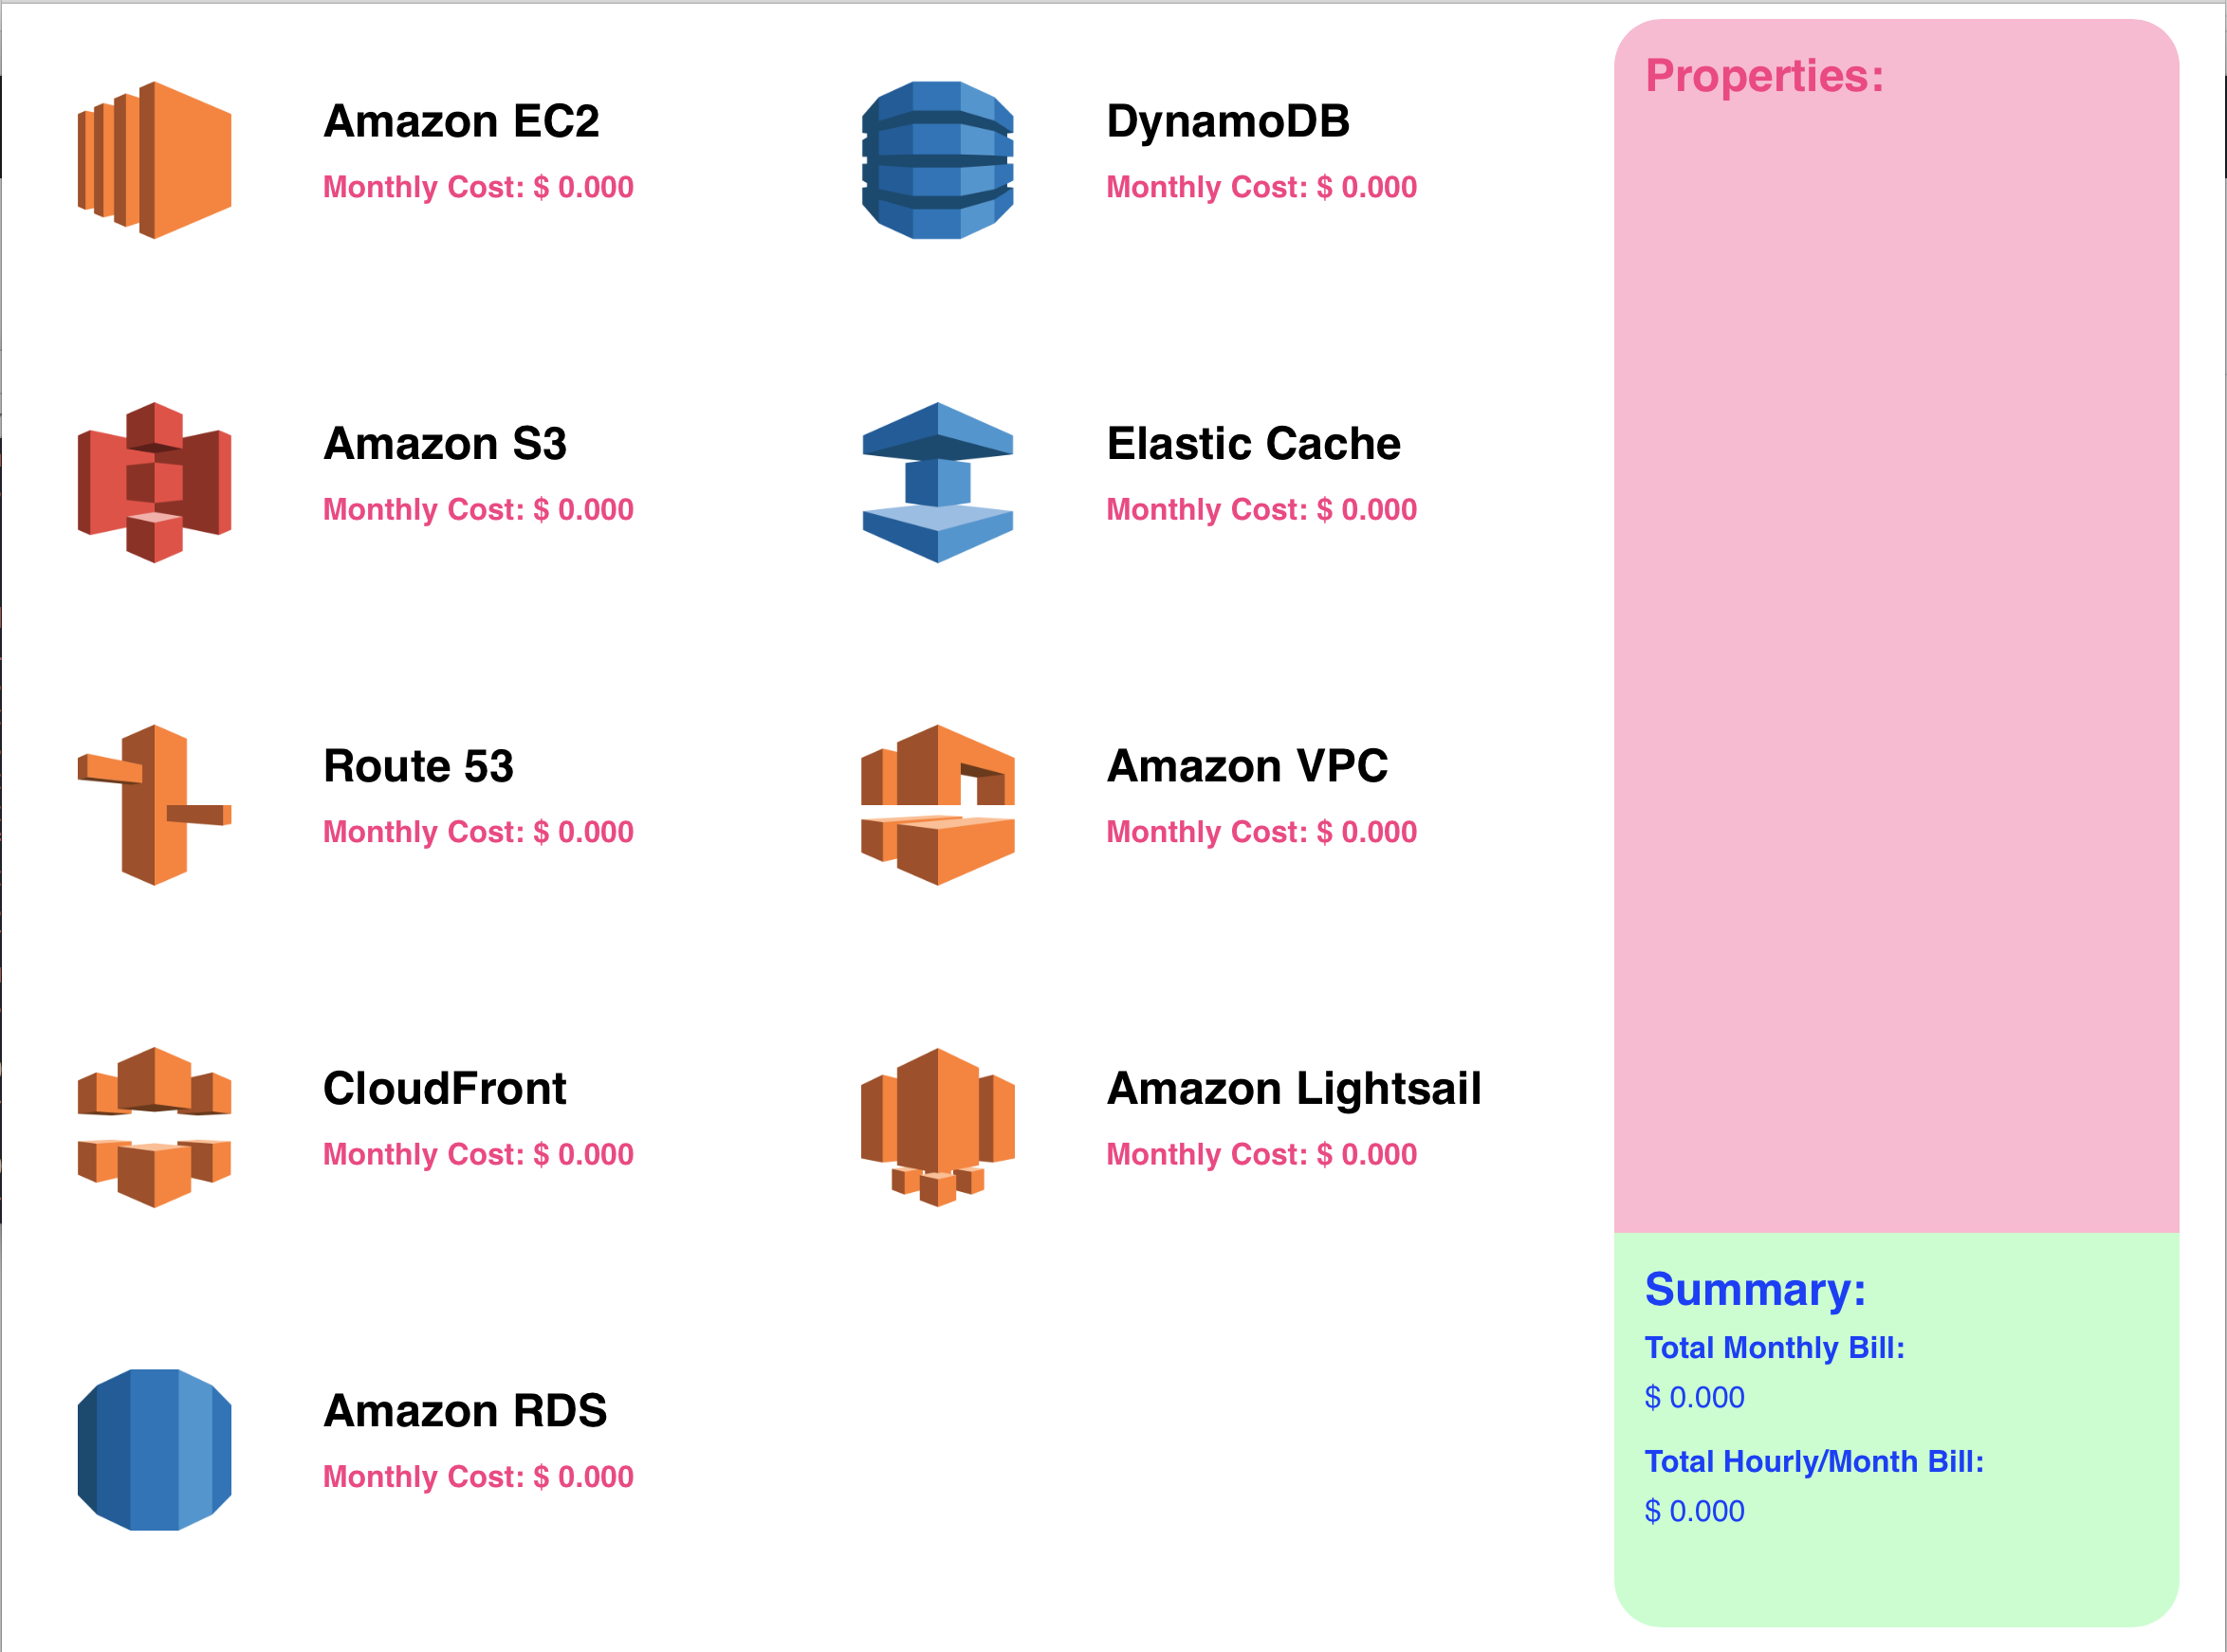
\includegraphics[width=15cm, height=10cm]{awspi.png}\\
  \caption[Tampilan Awal Aplikasi Berjalan]{Tampilan Awal Aplikasi Berjalan}
    \end{figure}

    \begin{figure}[H]
      \centering
  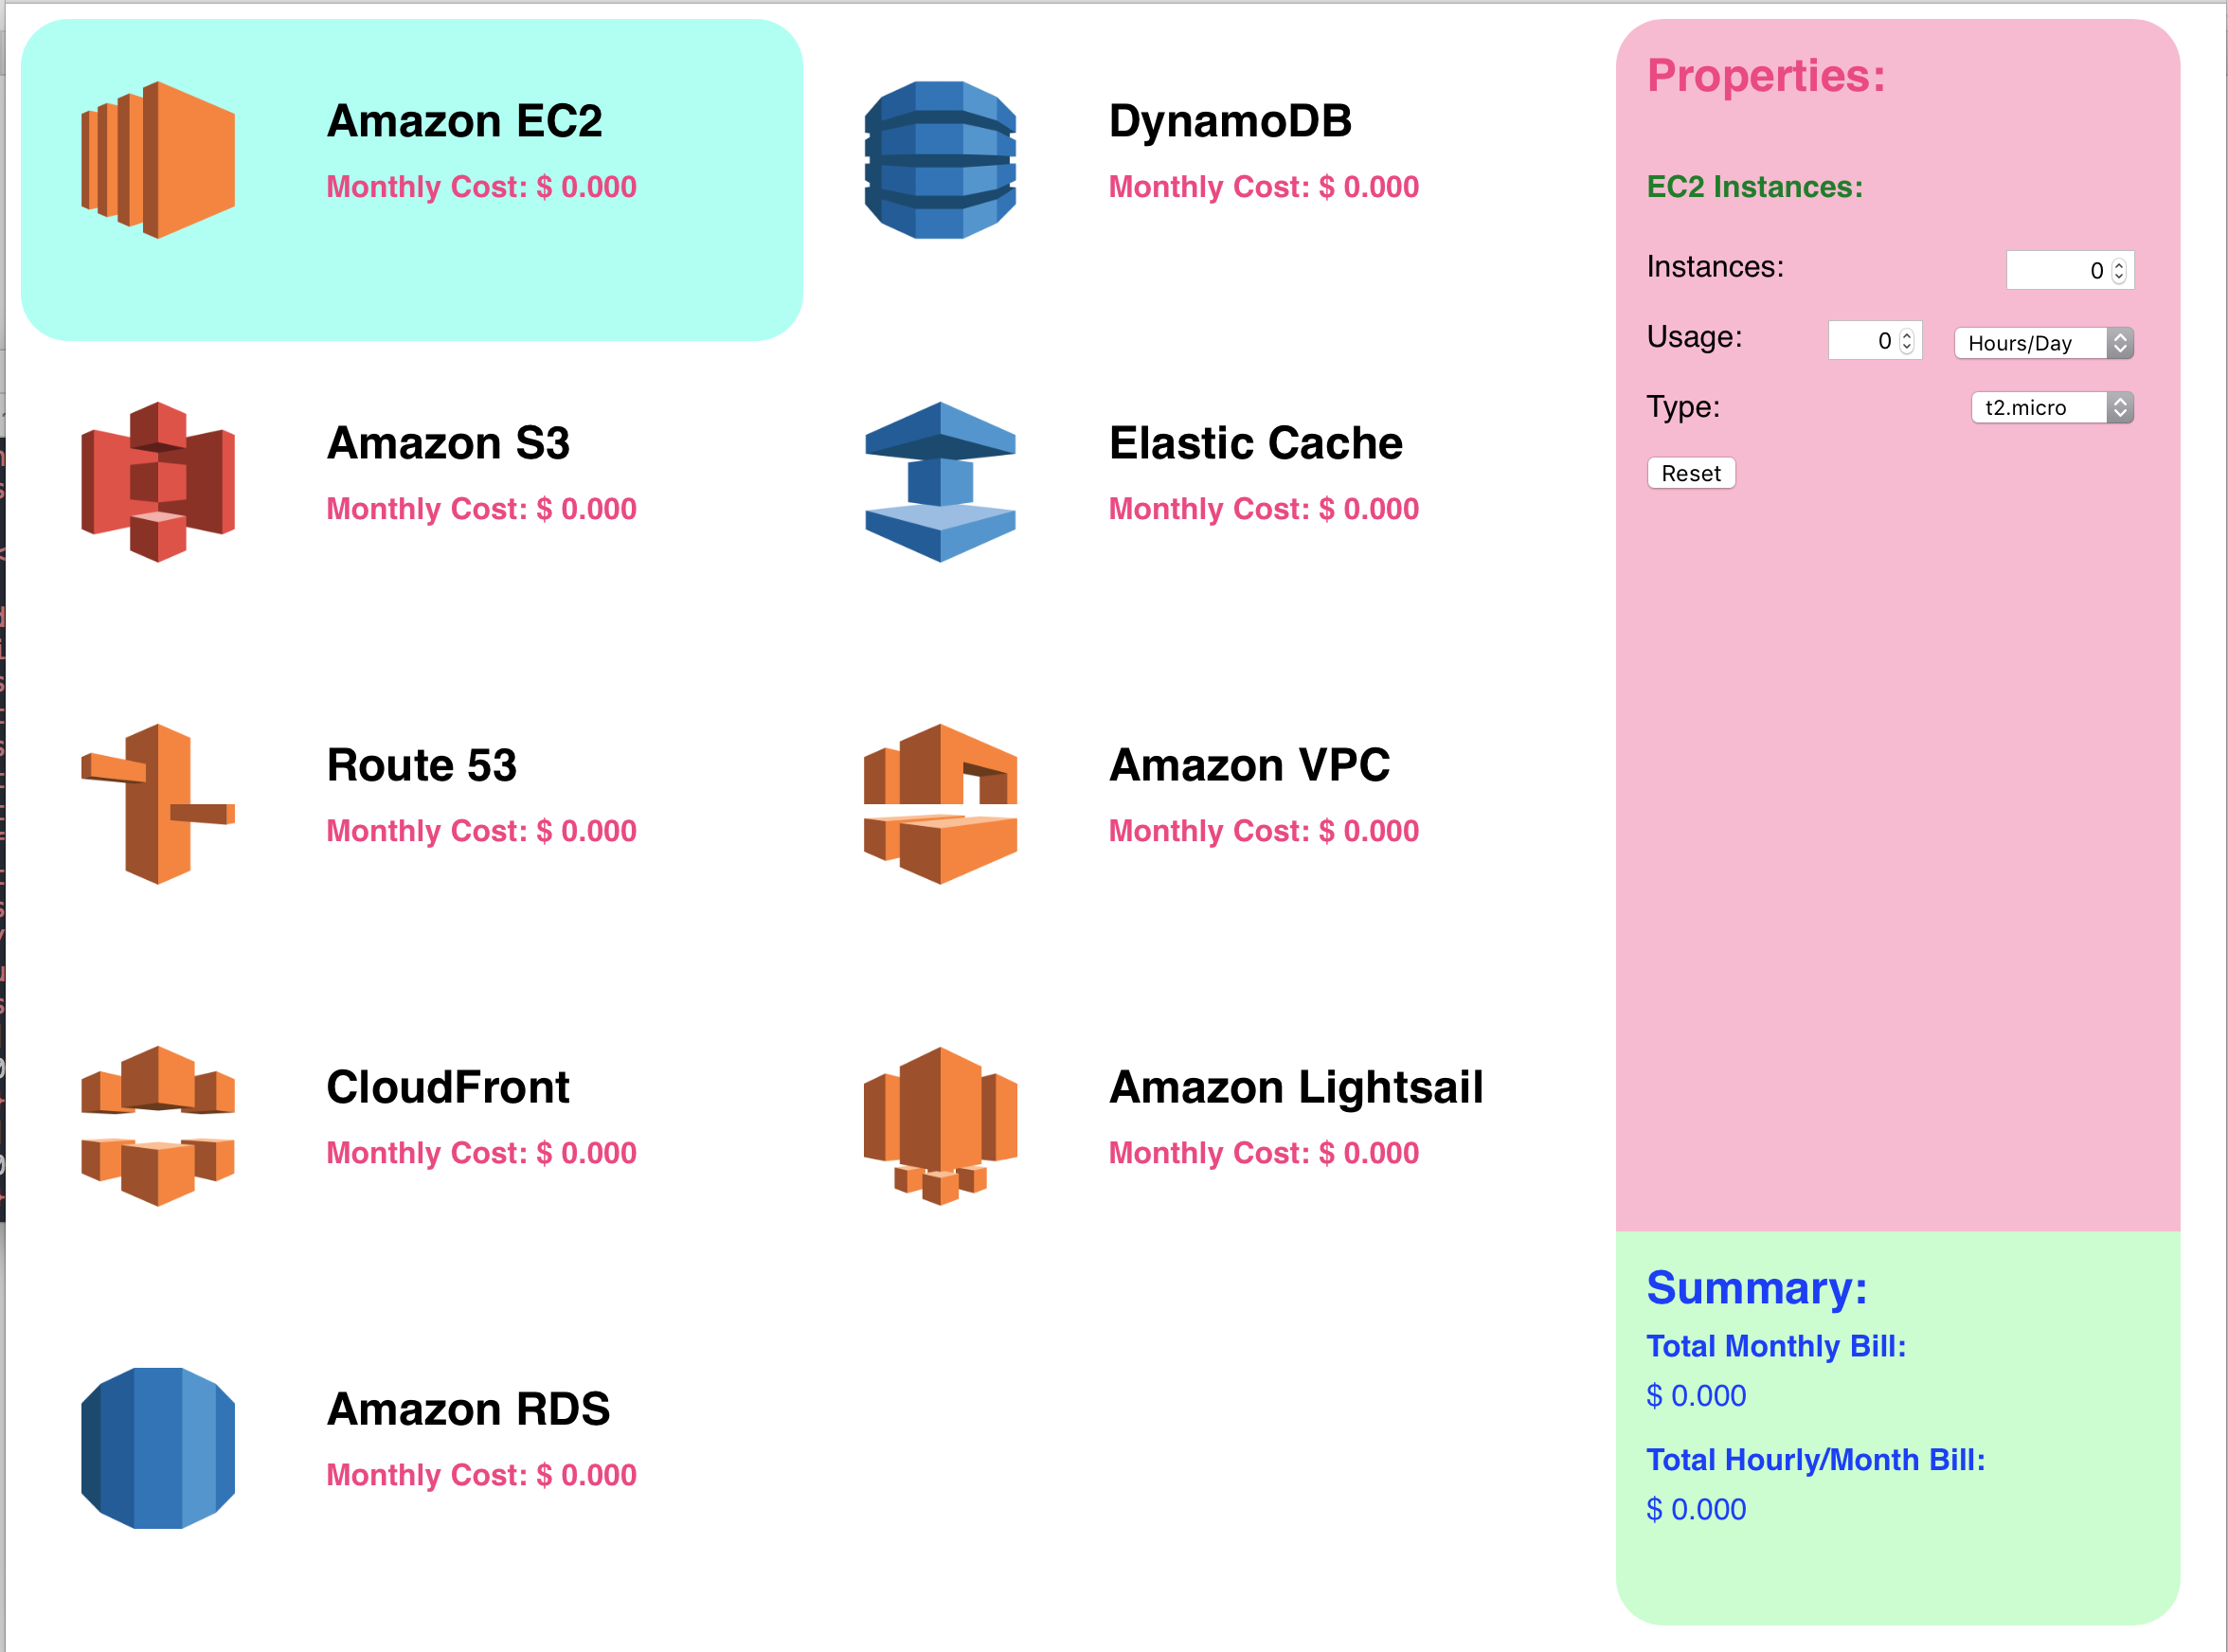
\includegraphics[width=15cm, height=10cm]{aws2.png}\\
  \caption[Tampilan Seleksi Menu]{Tampilan Ketika Salah Satu Menu Terseleksi}
    \end{figure}


\subsection{Algoritma Aplikasi}\hspace{5pt}
Dalam pembuatan aplikasi menggunakan bahasa Haskell, algoritma yang ada tidak berbeda jauh dengan algoritma yang digunakan dalam membuat sebuah aplikasi pada bahasa pemrograman lainnya. Pada penulisan kali ini, Aplikasi pertama kali dijalankan melalui fungsi \fhaskell{main} yang ada pada file \fhaskell{Main.hs}. File \fhaskell{Main.hs} terletak di folder \url{./frontend/Main.hs} dimana tanda \fhaskell{' . '} pada susunan file sistem operasi OS X menandakan lokasi awal dimana program itu berada. Fungsi \fhaskell{main} pada file tersebut adalah:\\

  \begin{lstlisting}[language=Haskell]
    main :: IO ()
    main = runFile "index.html" "" mainWk
  \end{lstlisting}

  \hspace{5pt}Fungsi \fhaskell{main} memiliki tipe data \fhaskell{IO ()} sebagaimana telah disebutkan pada bab sebelumnya bahwa fungsi tersebut menandakan akan adanya kemungkinan interaksi pada dunia luar atau kemungkinan terjadinya proses perubahan data yang bersifat \emph{mutable}. Pada Aplikasi, fungsi \fhaskell{main} merupakan hasil operasi dari fungsi runFile, yang memiliki tipe fungsi:\\

    \begin{lstlisting}[language=Haskell]
  runFile :: ByteString -- ^ The file to navigate to.
        -> ByteString -- ^ The path to allow read access to.
        -> JSM ()
        -> IO ()
    \end{lstlisting}

    \hspace{5pt}Seperti telah dijelaskan dalam bab sebelumnya, bahwa pada saat fungsi \fhaskell{runFile} dipanggil, fungsi \fhaskell{runFile} akan menerima input parameter pertama dan kedua dengan tipe data \fhaskell{ByteString} berupa \fhaskell{"index.html"} sebagai parameter pertama dan \fhaskell{" "} sebagai parameter kedua. Dalam pembuatan program dengan bahasa Haskell, alat kompilasi dapat menyesuaikan suatu tipe data yang merupakan tipe data bawaan Haskell. Sebagai contoh dalam penentuan apakah tipe data \fhaskell{"index.html"} adalah sebuah tipe data \fhaskell{String} atau tipe data \fhaskell{ByteString}. Dari potongan kode diatas, alat kompilasi akan secara otomatis mengetahui berdasarkan tipe data yang didefinisikan oleh fungsi \fhaskell{runFile} yaitu \fhaskell{ByteString} sehingga walaupun \fhaskell{"index.html"} juga bisa dikategorikan sebagai \fhaskell{String}, namun alat kompilasi akan mendeteksinya sebagai \fhaskell{ByteString}.

    \hspace{5pt}Pada fungsi \fhaskell{main}, parameter kedua yang menandakan letak lokasi pada parameter pertama. Dengan parameter aktual berupa \fhaskell{" "}, maka hal ini menandakan bahwa lokasi dari parameter pertama yaitu file \fhaskell{index.html} berada pada lokasi yang sama dengan lokasi tempat \emph{binary} file program berada nantinya atau dapat dikatakan bahwa lokasi file \fhaskell{index.html} akan mengikuti lokasi tempat \emph{binary} program berada. 

    \hspace{5pt}Argumen ketiga fungsi \fhaskell{runFile} yaitu \fhaskell{JSM ()} merupakan sebuah tipe data monadik yang menandakan bahwa parameter ketiga tersebut harus berada pada notasi monadik \fhaskell{JSM} dan parameter tersebut akan dikompilasi dengan menggunakan alat kompilasi GHC. Pada kode yang terdapat dalam fungsi \fhaskell{main}, parameter ketiga tersebut merupakan fungsi \fhaskell{mainWk} yang ada pada file \fhaskell{Main.hs} dimana tempat \emph{widget} yang digunakan untuk membangun Aplikasi.

    \hspace{5pt}Pada potongan kode diatas, fungsi \fhaskell{mainWk} memiliki tipe data \fhaskell{JSM ()}, yang merupakan hasil dari fungsi \fhaskell{mainWidgetWithHead}. Fungsi \fhaskell{mainWidgetWithHead} merupakan salah satu fungsi bawaan pustaka reflex-dom yang memiliki tipe fungsi:\\
   \begin{lstlisting}[language=Haskell]
      mainWidgetWithHead ::
          Widget Spider (Gui Spider (WithWebView SpiderHost) (HostFrame Spider)) () ->
          Widget Spider (Gui Spider (WithWebView SpiderHost) (HostFrame Spider)) () -> IO ()
   \end{lstlisting}

   \hspace{5pt}Dari potongan kode diatas, dapat diketahui bahwa fungsi \fhaskell{mainWidgetWithHead} memerlukan 2 (dua) buah parameter masukan yang keduanya memiliki tipe data \fhaskell{Widget Spider (Gui Spider (WithWebView SpiderHost) (HostFrame Spider)) ()}. Parameter ini berupa parameter bertipe data \fhaskell{Widget} yang berfungsi untuk membangun \emph{widget} pada Aplikasi. Pada file \fhaskell{Main.hs}, 2 (dua) buah parameter pada fungsi \fhaskell{mainWidgetWithHead} adalah berupa fungsi \fhaskell{headElement} dan \fhaskell{bodyElement}. Kedua fungsi tersebut merupakan fungsi yang akan menghasilkan \emph{widget} berupa DOM untuk ditranslasikan kedalam format HTML ketika nantinya Aplikasi dijalankan.

   \hspace{5pt}Setelah fungsi \fhaskell{main} dijalankan, maka secara otomatis fungsk \fhaskell{mainWK} akan dipanggil. Pada fungsi \fhaskell{mainWk}, fungsi utama yang membuat tampilan awal Menu Utama, Menu Properti dan Menu Summary pada saat Aplikasi pertama kali dijalankan adalah fungsi \fhaskell{bodyElement}. Isi dari fungsi \fhaskell{bodyElement} dapat dilihat pada potongan kode:\\
   
   \begin{lstlisting}[language=Haskell]
     bodyElement :: MonadWidget t m => m ()
     bodyElement = elClass "div" "container" $ do
      rec
       midM <- elClass "div" "middleMenu" $ do
         rec
          ...
       rightM <- elClass "div" "rightMenu" $ do
         rec
          ...
       elClass "div" "summaryMenu" $ do
         ...
      return ()
   \end{lstlisting}

   \hspace{5pt}Dari potongan kode diatas, diketahui bahwa fungsi \fhaskell{bodyElement} terbagi menjadi 3 bagian utama yang berupa variabel, yaitu variabel \fhaskell{midM}, variabel \fhaskell{rightM} dan sebuah ekspresi pada fungsi \fhaskell{elClass "div" "summaryMenu"} dan diakhiri dengan fungsi \fhaskell{return} yang mengambil parameter berupa \fhaskell{()} atau biasa disebut dengan \emph{unit}.

   \hspace{5pt}Dengan dijalankannya fungsi \fhaskell{return} tersebut, maka rangkaian eksekusi dari fungsi tersebut akan memiliki nilai keluaran bertipe data \fhaskell{IO ()}. Hal ini sesuai dengan hasil dari keluaran yang diharapkan pada fungsi \fhaskell{bodyElement} yaitu \fhaskell{m ()} karena tipe data \fhaskell{m} pada Haskell bersifat polimorfis sehingga tipe data \fhaskell{IO} dapat dikategorikan oleh alat kompilasi sebagai bagian dari tipe data \fhaskell{m} tersebut.

   \hspace{5pt}Dari ketiga bagian fungsi \fhaskell{bodyElement}, maka yang pertama kali dijalankan oleh fungsi tersebut adalah menentukan isi dari variabel \fhaskell{midM}, dimana fungsi ini akan menghasilkan tampilan utama Aplikasi, yaitu berupa tampilan Menu Utama yang berisi ikon-ikon jasa AWS berupa logo, nama jasa serta total perhitungan biaya sementara. Ikon-ikon ini nantinya berfungsi untuk menentukan tampilan properti jasa AWS mana yang akan ditampilkan pada Menu Properti ketika ditekan.

   \subsubsection{Variabel \fhaskell{midM} Sebagai Pembangun Menu Utama}\hspace{10pt}
   Variabel \fhaskell{midM} merupakan variabel yang mendefiniskan hasil dari tampilan Menu Utama. Contoh dari tampilan tersebut terdapat pada Gambar 3.18.

  \begin{figure}[H]
    \centering
  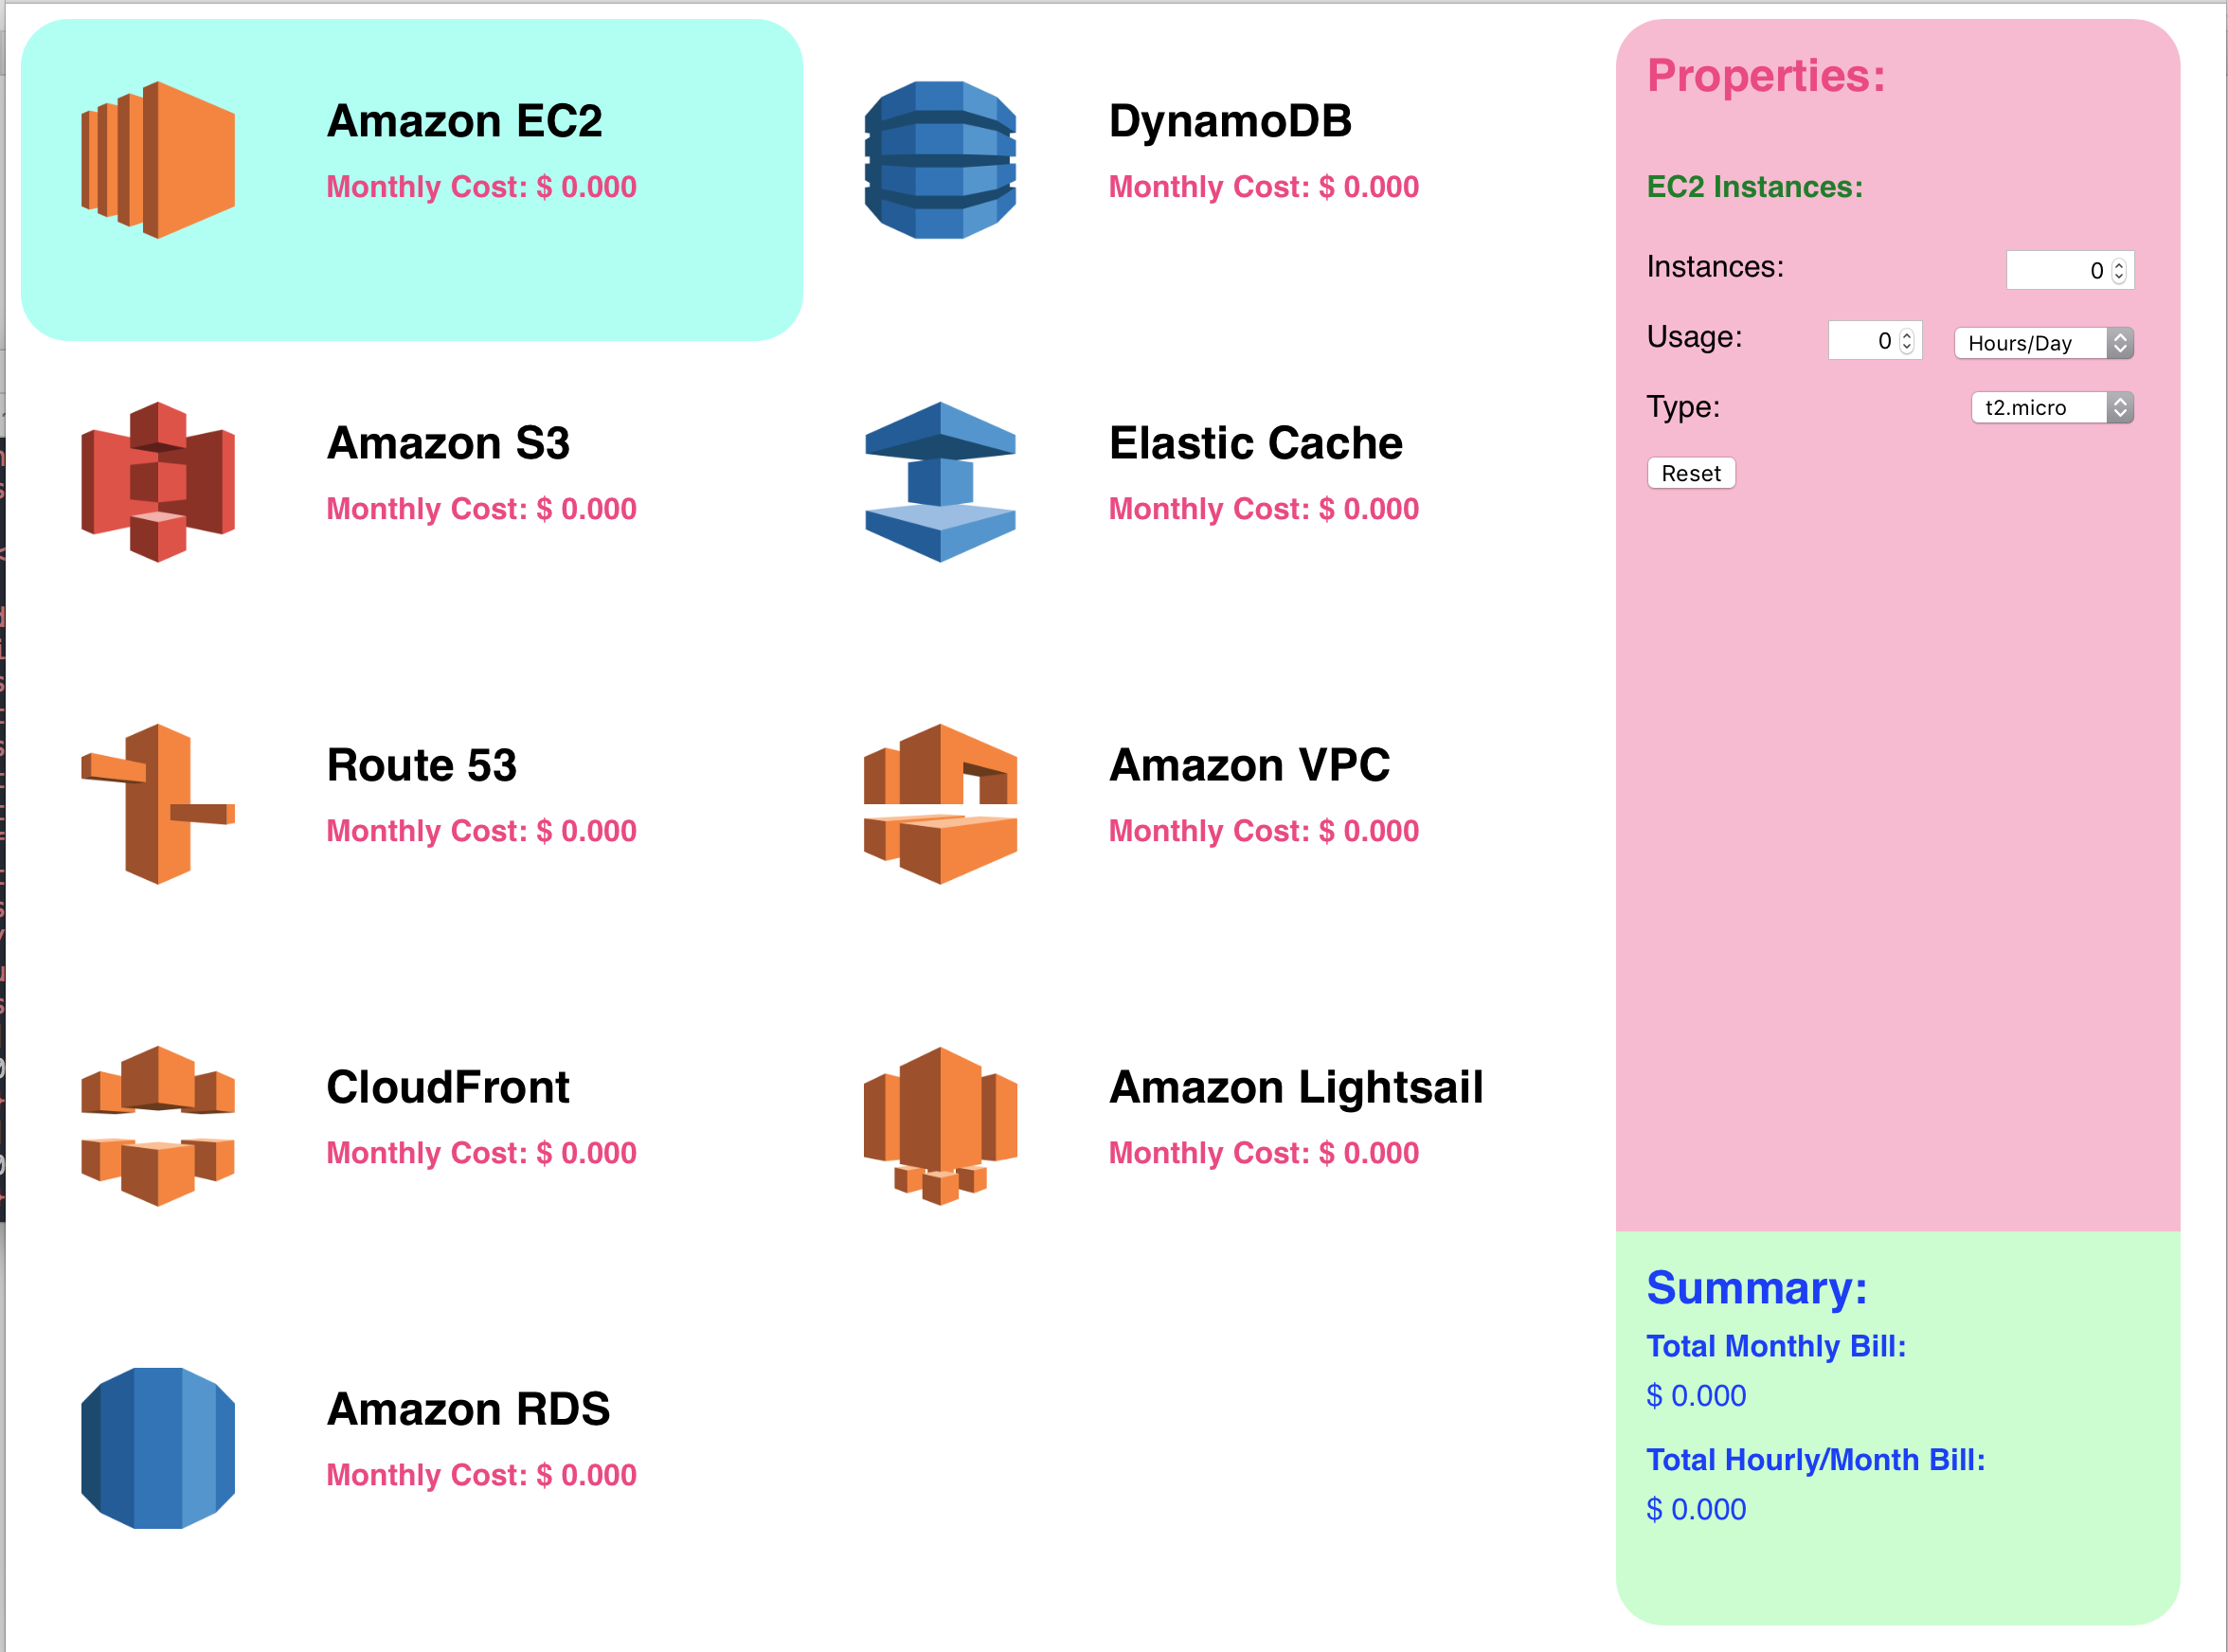
\includegraphics[width=15cm, height=10cm]{aws2.png}
  \caption[Tampilan Menu Dipilih]{Tampilan Aplikasi Saat Menu Dipilih}
  \end{figure}

  \hspace{10pt}Isi dari variabel \fhaskell{midM} dapat dilihat pada kode: \\
     \begin{lstlisting}[language=Haskell]
       midM <- elClass "div" "middleMenu" $ do
             rec
              ec2 <- serviceButton "Amazon EC2" EC2 ec2dynAttrs (theDynCost rightM 1)
              s3  <- serviceButton "Amazon S3" S3 s3dynAttrs (theDynCost rightM 2)
              r53 <- serviceButton "Route 53" R53 r53dynAttrs (theDynCost rightM 3)
              cf  <- serviceButton "CloudFront" CF cfdynAttrs (theDynCost rightM 4)
              rds <- serviceButton "Amazon RDS" RDS rdsdynAttrs (theDynCost rightM 5)
              db  <- serviceButton "DynamoDB" DB dbddynAttrs (theDynCost rightM 6)
              ec  <- serviceButton "Elastic Cache" EC ecdynAttrs (theDynCost rightM 7)
              vpc <- serviceButton "Amazon VPC" VPC vpcdynAttrs (theDynCost rightM 9)
              ls  <- serviceButton "Amazon Lightsail" LS lsdynAttrs (theDynCost rightM 10)

              let 
	          ec2dynAttrs = labelAttrs <$> curSelect dynSelect EC2
	          s3dynAttrs  = labelAttrs <$> curSelect dynSelect S3
	          r53dynAttrs = labelAttrs <$> curSelect dynSelect R53
	          cfdynAttrs  = labelAttrs <$> curSelect dynSelect CF
	          rdsdynAttrs = labelAttrs <$> curSelect dynSelect RDS
	          dbddynAttrs = labelAttrs <$> curSelect dynSelect DB
	          ecdynAttrs  = labelAttrs <$> curSelect dynSelect EC
	          vpcdynAttrs = labelAttrs <$> curSelect dynSelect VPC
	          lsdynAttrs  = labelAttrs <$> curSelect dynSelect LS
              dynSelect <- holdDyn Nothing $ Just <$> leftmost [ec2, s3, r53, cf, rds, db, ec, vpc, ls]
             return dynSelect
     \end{lstlisting}

     \hspace{10pt}Seperti yang telah dijelaskan dalam bab sebelumnya, bahwa variabel pada Haskell hanyalah sebagai identifikasi nama dan bukan tempat penampung suatu nilai. Variabel \fhaskell{midM} pada potongan kode dibawah ini adalah sebuah identifikasi atas hasil dari fungsi \fhaskell{elClass} yang dilekatkan pada variabel \fhaskell{midM} menggunakan fungsi \fhaskell{($<$-)} atau yang biasa dikenal sebagai fungsi pengikat (\emph{binding function}). Fungsi \fhaskell{($<$- )} merupakan \emph{binding arrow} dimana \fhaskell{midM} merupakan identifikasi yang didalamnya terkandung nilai dari hasil eksekusi kode setelah tanda \fhaskell{( $<$- )}.

     \hspace{10pt}Fungsi yang dijalankan untuk menentukan isi dari \fhaskell{midM} adalah fungsi \fhaskell{elClass} yang memiliki tipe data \fhaskell{elClass :: Text -> Text -> m t a -> m t a}. Dikarenakan bahasa pemrograman Haskell merupakan bahasa fungsional yang memiliki konsep \emph{High Order Function} dimana parameter sebuah fungsi dapat berupa fungsi lain, maka pada fungsi \fhaskell{elClass} diatas, parameter ketiga berupa \fhaskell{m a} dapat berupa sebuah fungsi, yaitu yang diawali dengan penggunaan notasi \fhaskell{do} dan diakhiri dengan dijalankannya fungsi \fhaskell{return dynSelect}. Pada penulisan ini, yang akan dijadikan contoh penjelasan hanya 1 (satu) variabel yaitu \fhaskell{ec2} dan \fhaskell{ec2dynAttrs}

     \hspace{10pt}Ketika menggunakan notasi \fhaskell{do}, potongan kode diatas juga menggunakan fungsi \fhaskell{rec} (lihat pada potongan kode dibawah), yaitu suatu fungsi rekursif pada notasi \fhaskell{do} yang digunakan untuk membuat variabel dapat digunakan sebelum didefinisikan. Hal ini memungkinkan karena bahasa Haskell bersifat \emph{lazy}, yaitu variabel akan dijalankan ketika dibutuhkan saja. Hal ini dilakukan alat kompilasi ketika melakukan kompilasi kode Haskell.\\

\begin{lstlisting}[language=Haskell]
elClass "div" "middleMenu" $ do
  rec
    ...
    ...
\end{lstlisting}

     \hspace{10pt}Notasi \fhaskell{do} pada fungsi \fhaskell{elClass} kemudian mendefinisikan masing-masing ikon pada Menu Utama yang akan tampil berupa variabel \fhaskell{ec2}, \fhaskell{s3}, \fhaskell{r53}, \fhaskell{cf}, \fhaskell{rds}, \fhaskell{db}, \fhaskell{ec}, \fhaskell{vpc}, \fhaskell{ls} sebagai inisial dari dari masing-masing jasa AWS. Sama seperti pada variabel \fhaskell{midM}, masing-masing variabel tersebut merupakan definisi dari hasil fungsi \fhaskell{serviceButton} yang memiliki tipe dan isi fungsi:\\
\begin{lstlisting}[language=Haskell]
serviceButton :: (MonadWidget t m) => T.Text
                                   -> AwsIcon
				   -> Dynamic t (Map.Map T.Text T.Text)
				   -> Dynamic t T.Text
				   -> m (Event t AwsIcon)
serviceButton label icon dynAttrs dynCost = do
    (ev1,_) <- elDynAttr' "label" ((constDyn $ idAttrs icon) <> dynAttrs) $ do
            elAttr' "img" (imgAttrs icon) $ text ""
            el "h2" $ text label
	    let text1 = constDyn "Monthly Cost: $ "
            el "h4" $ dynText $ text1 <> dynCost
    return $ icon <$ (domEvent Click ev1)
\end{lstlisting}
\pagebreak
\hspace{10pt}Fungsi \fhaskell{serviceButton} pada potongan kode sebelumnya memerlukan 4 (empat) parameter yaitu:

\begin{enumerate}[leftmargin=1.65cm]
\item Parameter pertama (\fhaskell{label}) adalah parameter bertipe data \fhaskell{Text} yang berguna sebagai nama dari jasa AWS yang akan tampil pada Menu Utama. Parameter ini digunakan sebagai isi dari elemen \fhaskell{h2} pada HTML yaitu elemen yang menandakan sebuah \emph{header}. Parameter ini digunakan pada potongan kode \fhaskell{el "h2" \$ text label}
\item Parameter kedua (\fhaskell{icon}) adalah parameter bertipe \fhaskell{AwsIcon} dimana parameter ini adalah tipe data buatan yaitu tipe data:\\
  \begin{lstlisting}[language=Haskell]
    data AwsIcon = CF | DB | EC2 | EC | LS | RDS | R53 | S3 | VPC
    deriving (Eq, Show, Ord)
  \end{lstlisting}
  parameter \fhaskell{icon} ini akan digunakan untuk nilai kembalian pada tipe data keluaran fungsi \fhaskell{serviceButton} yaitu \fhaskell{m (Event t AwsIcon)}. Hal ini terdapat dalam baris kode \fhaskell{return $ icon <$ (domEvent Click ev1)}.
\item Parameter ketiga  (\fhaskell{dynAttrs}) adalah parameter bertipe data \fhaskell{Dynamic t (Map.Map T.Text T.Text)} yaitu sebuah tipe data \fhaskell{Map} yang bersifat dinamis. Parameter ini akan menentukan \emph{icon} Menu Utama yang dipilih oleh pengguna.

\item Parameter keempat (\fhaskell{dynCost}) adalah parameter bertipe data \fhaskell{Dynamic t T.Text} yang digunakan sebagai tampilan harga sementara pada setiap \emph{icon} jasa AWS pada Menu Utama. Harga sementara ini dibungkus kedalam tipe data \fhaskell{Dynamic} yang menandakan bahwa nilai yang terkandung dalam tipe data tersebut dapat berubah-ubah seiring waktu.
\end{enumerate}

\hspace{10pt}Implementasi fungsi \fhaskell{serviceButton} adalah pada salah satu baris yaitu \fhaskell{ec2 <- serviceButton "Amazon EC2" EC2 ec2dynAttrs (theDynCost rightM 1)} dimana pada baris ini, fungsi \fhaskell{serviceButton} menerima parameter aktual berupa \fhaskell{Amazon EC2}, \fhaskell{EC2}, \fhaskell{ec2dynAttrs}, \fhaskell{(theDynCost rightM 1)}. Dari potongan kode tersebut, maka dapat dilihat bahwa salah satu keunggulan Haskell pada \emph{lazy evaluation} terletak pada penggunaan parameter \fhaskell{ec2dynAttrs} dan \fhaskell{(theDynCost rightM 1)} yang belum didefinisikan sebelumnya. Hal ini juga merupakan keunggulan dari \emph{RecursiveDo} yang dimiliki oleh Haskell sehingga memungkinkannya fungsi \fhaskell{ec2dynAttrs} didefinisikan setelah fungsi \fhaskell{servickeButton}.

\hspace{10pt}Pada variabel \fhaskell{midM}, eksekusi terakhir sehingga menjadikan \fhaskell{midM} selesai terdefinisi terdapat pada baris \fhaskell{return dynSelect}. Variabel \fhaskell{dynSelect} sebagai parameter dari fungsi \fhaskell{return} merupakan hasil dijalankannya fungsi \fhaskell{holdDyn} yang berisikan nilai dari hasil variabel \fhaskell{ec2}, \fhaskell{s3}, \fhaskell{r53}, \fhaskell{cf}, \fhaskell{rds}, \fhaskell{db}, \fhaskell{ec}, \fhaskell{vpc}, \fhaskell{ls}. Hal tersebut dapat dilihat dari potongan kode program:\\
\begin{lstlisting}[language=Haskell]
dynSelect <- holdDyn Nothing $ Just <$> leftmost [ec2, s3, r53, cf, rds, db, ec, vpc, ls]
return dynSelect
\end{lstlisting}

\hspace{10pt}Dari potongan kode diatas, hasil dari fungsi \fhaskell{serviceButton} yang terdefinisi didalam masing-masing variabel ditempatkan kedalam sebuah \fhaskell{list} dan \fhaskell{list} tersebut kemudian diaplikasikan oleh fungsi \fhaskell{leftmost} dengan perantara fungsi \fhaskell{(<\$>}). Fungsi \fhaskell{leftmost} berguna sebagai acuan program atas tombol mana yang ditekan terlebih dahulu oleh pengguna. Sehingga, apabila tombol pada icon EC2 ditekan, maka \fhaskell{midM} akan menghasilkan sebuah tipe data \fhaskell{Dynamic t (Maybe AwsIcon)}, dimana nilai dari \fhaskell{AwsIcon} pada tipe data tersebut adalah \fhaskell{EC2}.


\subsubsection{Variabel \fhaskell{rightM} Sebagai Pembangun Menu Properti}\hspace{10pt}
  Fungsi midM kemudian mengirimkan hasil seleksi secara dinamis tersebut kedalam fungsi rightM, sehingga tampilan pada sisi kanan aplikasi akan berubah seketika setelah menu utama dipilih. Tampilan rightM adalah tampilan properties dari jasa EC2 pada AWS yang digunakan untuk munentukan hasil estimasi biaya yang harus dikeluarkan. Hasil dari kalkulasi ini akan digunakan untuk menentukan total biaya untuk ditampilkan pada summary menu dan pada setiap icon sesuai dengan properti masing-masing icon. Isi dari kode pada rightM adalah:\\
     
   \begin{lstlisting}[language=Haskell]
    rightM <- elClass "div" "rightMenu" $ do
               el "h2" $ text "Properties: "
               rec
                ec2Prop <- ec2Properties ec2dynAttrs
                s3Prop  <- s3Properties s3dynAttrs
                r53Prop  <- r53Properties r53dynAttrs
                cfProp  <- cfProperties cfdynAttrs
                rdsProp  <- rdsProperties rdsdynAttrs
                dbProp  <- dbProperties dbdynAttrs
                ecProp  <- ecProperties ecdynAttrs
                vpcProp  <- vpcProperties vpcdynAttrs
                lsProp  <- lsProperties lsdynAttrs
      
                let 
	                ec2dynAttrs = showAttrs <$> curSelect midM EC2
	                s3dynAttrs  = showAttrs <$> curSelect midM S3
	                r53dynAttrs = showAttrs <$> curSelect midM R53
	                cfdynAttrs  = showAttrs <$> curSelect midM CF
	                rdsdynAttrs = showAttrs <$> curSelect midM RDS
	                dbdynAttrs  = showAttrs <$> curSelect midM DB
	                ecdynAttrs  = showAttrs <$> curSelect midM EC
                  vpcdynAttrs = showAttrs <$> curSelect midM VPC
	                lsdynAttrs  = showAttrs <$> curSelect midM LS
               return [ (1 , ec2Prop)
	                    , (2 , s3Prop )
	                    , (3 , r53Prop)
		                  , (4 , cfProp )
		                  , (5 , rdsProp)
		                  , (6 , dbProp )
		                  , (7 , ecProp )
		                  , (8 , vpcProp)
		                  , (9 , lsProp )
		                  ]
   \end{lstlisting}

   \hspace{10pt}Dari kode diatas, properti dari masing-masing tombol \emph{icon} pada menu yang dihasilkan dari fungsi \fhaskell{elClass} pada variabel \fhaskell{midM} ditentukan oleh atribut dari:\\

  \begin{lstlisting}[language=HTML]
  <div class="rightProp" id="EC2" style="display:none">...</div>
  \end{lstlisting}
  Menu Properti akan muncul seiring dengan tombol mana yang ditekan oleh pengguna sesuai dengan atribut \fhaskell{display} dimana tampilan properti jasa AWS yang aktif tersebut akan muncul dengan diubahnya \fhaskell{'none'} menjadi \fhaskell{'inline-flex'} apabila \emph{output} dari fungsi \fhaskell{curSelect} yang diaplikasikan kepada variabel \fhaskell{midM} dan masing-masing icon bernilai \fhaskell{True}. Sehingga fungsi:\\

  \begin{lstlisting}[language=Haskell]
  showAttrs :: Bool -> Map.Map T.Text T.Text
  showAttrs b = "style" =: ("display: " <> display' b)
  where
    display' True = "inline-flex"
    display' _    = "none"
  \end{lstlisting}
  yang diaplikasikan terhadap hasil dari fungsi \fhaskell{curSelect} tersebut merubah atribut \emph{style} dengan nilai \emph{display} secara dinamis sesuai dengan keadaan dimana tombol icon AWS pada variabel \fhaskell{midM} sedang ditekan.

  \hspace{10pt}Dengan demikian, setiap properti yang diubah akan membawa suatu hasil yang berbeda sesuai keadaan terakhir nilai dari masing-masing properti tersebut. Variabel \fhaskell{rightM} akan membawa sebuah nilai hasil dari perhitungan masing-masing properti pada icon AWS dengan melakukan pemetaan berupa hashmap, yaitu sebuah pemetaan yang setiap nilai dari suatu variabel ditandai dengan kunci-kunci yang mencirikan variabel tersebut. Seperti contoh pada kode program:\\
    \begin{lstlisting}[language=Haskell]
  return [ (1 , ec2Prop)
	       , (2 , s3Prop )
	       , (3 , r53Prop)
		     , (4 , cfProp )
		     , (5 , rdsProp)
		     , (6 , dbProp )
		     , (7 , ecProp )
		     , (8 , vpcProp)
		     , (9 , lsProp )
		     ]
    \end{lstlisting}

   \hspace{10pt} Dari potongan kode diatas, \fhaskell{rightM} akan membawa sebuah nilai dinamis (\emph{dynamic values} yang memiliki kunci dari 1 sampai 9 untuk menandakan masing-masing properti (misalnya: kunci 1 untuk variabel \fhaskell{ec2Prop}, yaitu hasil dari perhitungan properti pada saat tombol ikon EC2 ditekan). Nilal kembalian ini akan digunakan oleh \fhaskell{midM} untuk menampilkan total biaya pada setiap ikonnya. Hal ini dimungkinkan karena adanya fungsi \fhaskell{rec} pada notasi \fhaskell{do} pada fungsi \fhaskell{bodyElement}.


\subsubsection{Menu Summary Sebagai Hasil Total Perhitungan Sementara}\hspace{10pt}
   Kemudian hasil dari kalkulasi tersebut akan ditampilkan pada menu summary yang terletak di sisi kanan bawah pada gambar diatas. Hasil kalkulasi tersebut diperoleh dari penjumlahan seluruh properti yang telah dihitung sesuai dengan ketentuan harga yang diberikan oleh situs dokumentasi AWS yang resmi. Isi dari kode pada \fhaskell{elClass "div" "summaryMenu"}  adalah:\\ 
   \begin{lstlisting}[language=Haskell]
let
        resultList = (fmap . fmap) readDouble (Map.elems $ Map.fromList rightM)
	starter = readDouble <$> (constDyn "0")
	joined = join $ foldM foldTheCost starter resultList
      el "h2" $ text "Summary: "
      el "h4" $ text "Total Monthly Bill: "
      -- This is how foldM will work:
      --
      -- foldM f Dynamic t 0 [Dynamic t 5, Dynamic t 6]
      -- do
      --   a2 <- f (Dynamic t 0) (Dynamic t 5)
      --   a3 <- f (Dynamic t 5) (Dynamic t 6)
      --
      el "p" $ dynText $ (constDyn "$ ") <> (toText <$> (join $ foldM foldTheCost starter resultList))
      el "h4" $ text "Total Hourly/Month Bill: "
      el "p" $ dynText $ (constDyn "$ ") <> (toText <$> ((/720) <$> joined))
   \end{lstlisting}

  Kode yang menghitung total keseluruhan dari biaya masing-masing menu adalah:\\
     \begin{lstlisting}[language=Haskell]
  el "p" $ dynText $ (constDyn "$ ") <> (toText <$> (join $ foldM foldTheCost starter resultList))
     \end{lstlisting}

     dimana berguna untuk menggabungkan perhitungan dari setiap hasil kalkulasi yang dilakukan secara dinamis melalui fungsi \fhaskell{foldTheCost}. Sehingga, perubahan yang terjadi pada properti dari masing-masing menu yang secara seketika diperbaharui akan turut melakukan pembaharuan terhadap nilai jumlah biaya yang tertera pada teks "Total Hourly/Month Bill" dan "Total Monthly Bill: " pada Menu Summary.

     
\section{Hasil Uji Coba}
Pada penelitian ilmiah ini, untuk memeriksa apakah hasil akhir Aplikasi dapat digunakan oleh pengguna akhir (\emph{end-user}) adalah dengan melakukan beberapa uji coba. Uji coba dilakukan dengan melihat beberapa parameter seperti yang telah dijelaskan dalam Bab 1 sebelumnya. Hasil uji coba pada penelitian ilmiah ini akan dijelaskan berikut ini.
\subsection{Uji Coba Tampilan dan Fungsional Aplikasi}\hspace{5pt}
Dari hasil yang dilakukan dengan cara menjalankan aplikasi dan mencocokannya dengan rancangan yang telah dibuat dalam subbab sebelumnya, maka didapati hasil sebagai berikut:
\begin{enumerate}
\item Tampilan properti jasa AWS telah sesuai dengan ikon yang aktif pada menu utama
\item Setiap penambahan / perubahan pada properti dari setiap ikon aktif akan merubah tampilan "Monthly Cost pada masing-masing ikon pada menu utama dan pada summary menu
\end{enumerate}

\subsection{Uji Coba Kesesuaian Pada Dokumentasi AWS}\hspace{5pt}
Pencocokan dengan dokumentasi AWS dengan membandingkan harga yang telah ditetapkan sebelumnya dan dicocokkan dengan Aplikasi, maka didapati hasil sebagai berikut:
\begin{enumerate}

\item Perhitungan harga telah sesuai dengan dokumentasi harga dari situs resmi Amazon AWS di \url{amazon.com}
\item Jumlah total harga pada summary menu telah sama dengan hasil penjumlahan harga dari masing-masing ikon pada menu utama

\hspace{5pt}Berdasarkan hasil uji coba yang dilakukan, maka dapat dilihat bahwa Aplikasi sudah siap digunakan oleh pengguna akhir untuk melakukan kalkulasi jasa AWS yang paling sering digunakan oleh pengembang.
\end{enumerate}

\end{document}
